%%%%%%%%%%%%%%%%%%%%%%%%%%%%%%%%%%%%%%%%%%%%%%%%%%
% Set document class
\documentclass[12pt]{article}

% Define packages
\usepackage{hyperref, url} 
\usepackage{graphicx,amsfonts,psfrag,layout,subcaption,array,longtable,lscape,booktabs,dcolumn,amsmath,amssymb,amssymb,amsthm,setspace,epigraph,chronology,color,colortbl,caption,wasysym,diagbox,natbib,colortbl,authblk,commath}
\usepackage[]{graphicx}\usepackage[]{color}
\usepackage[page]{appendix}
\usepackage[section]{placeins}
\usepackage[linewidth=1pt]{mdframed}
\usepackage[margin={1in}]{geometry} %1 inch margins

\title{Building State Capacity through Public Land Disposal: An Application of Matrix Completion for Counterfactual Prediction} 
\author[ ]{Jason Poulos\thanks{\emph{Address for correspondence:} Department of Political Science, 210 Barrows Hall \#1950, Berkeley, CA 94720-1950. \emph{Email:} \href{mailto:poulos@berkeley.edu}{\nolinkurl{poulos@berkeley.edu}}. I thank Sean Gailmard, Eric Schickler, Ross Mattheis, and Shom Mazumder for helpful comments. I acknowledge support of the National Science Foundation Graduate Research Fellowship (DGE 1106400). This work used the computer resources of Stampede2 at the Texas Advanced Computing Center (TACC) under an Extreme Science and Engineering Discovery Environment (XSEDE) startup allocation (TG-SES180010).}}
\affil[ ]{University of California, Berkeley}
\date{}
\setcounter{Maxaffil}{0}
\renewcommand\Affilfont{\itshape\small}

% Reference labels in the online appendix
\usepackage{xr}
\externaldocument{land-reform-sm}

% Footnotes stick at the bottom
\usepackage[bottom]{footmisc}

% Multicolumns for references

\usepackage{multicol}

% New footnote characters
\usepackage{footmisc}
\DefineFNsymbols{mySymbols}{{\ensuremath\dagger}{\ensuremath\ddagger}\S\P
   *{**}{\ensuremath{\dagger\dagger}}{\ensuremath{\ddagger\ddagger}}}
\setfnsymbol{mySymbols}

%Rm thanks dagger
\renewcommand\footnotemark{}
%\renewcommand\footnoterule{}

% New tabular environment
\usepackage{tabularx}
\newcolumntype{Y}{>{\raggedleft\arraybackslash}X}% raggedleft column X

% Define appendix 
\renewcommand*\appendixpagename{Appendix}
\renewcommand*\appendixtocname{Appendix}

% Position floats
\renewcommand{\textfraction}{0.05}
\renewcommand{\topfraction}{0.95}
\renewcommand{\bottomfraction}{0.95}
\renewcommand{\floatpagefraction}{0.35}
\setcounter{totalnumber}{5}

% Colors for highlighting tables
\definecolor{Gray}{gray}{0.9}

% Different font in captions
\newcommand{\captionfonts}{\scriptsize}

\makeatletter  % Allow the use of @ in command names
\long\def\@makecaption#1#2{%
  \vskip\abovecaptionskip
  \sbox\@tempboxa{{\captionfonts #1: #2}}%
  \ifdim \wd\@tempboxa >\hsize
    {\captionfonts #1: #2\par}
  \else
    \hbox to\hsize{\hfil\box\@tempboxa\hfil}%
  \fi
  \vskip\belowcaptionskip}
%\makeatother   % Cancel the effect of \makeatletter
 
% Set Spacing
\doublespacing

% Number assumptions
\newtheorem*{assumption*}{\assumptionnumber}
\providecommand{\assumptionnumber}{}
\makeatletter
\newenvironment{assumption}[2]
 {%
  \renewcommand{\assumptionnumber}{Assumption #1}%
  \begin{assumption*}%
  \protected@edef\@currentlabel{#1}%
 }
 {%
  \end{assumption*}
 }
\makeatother

% Macros
\newcommand{\Adv}{{\mathbf{Adv}}}       
\newcommand{\prp}{{\mathrm{prp}}}                  % How to define new commands 
\newcommand{\calK}{{\cal K}}
\newcommand{\outputs}{{\Rightarrow}}                
\newcommand{\getsr}{{\:\stackrel{{\scriptscriptstyle\hspace{0.2em}\$}}{\leftarrow}\:}}
\newcommand{\andthen}{{\::\;\;}}    %  \: \; for thinspace, medspace, thickspace
\newcommand{\Rand}[1]{{\mathrm{Rand}[{#1}]}}       % A command with one argument
\newcommand{\Perm}[1]{{\mathrm{Perm}[{#1}]}}       
\newcommand{\Randd}[2]{{\mathrm{Rand}[{#1},{#2}]}} % and with two arguments
\newcommand{\E}{\mathrm{E}}
\newcommand{\Var}{\mathrm{Var}}
\newcommand{\Cov}{\mathrm{Cov}}
\DeclareMathOperator*{\plim}{plim}
\newcommand\independent{\protect\mathpalette{\protect\independenT}{\perp}}
\def\independenT#1#2{\mathrel{\rlap{$#1#2$}\mkern2mu{#1#2}}}
\newcommand{\possessivecite}[1]{\citeauthor{#1}'s (\citeyear{#1})} 

%%%%%%%%%%%%%%%%%%%%%%%%%%%%%%%%%%%%%%%%%%%%%%%%%%%%%%%%%%%%%%%%%%%%%%%%%%%%

\begin{document} 
 
\begin{singlespacing}
\maketitle  
\end{singlespacing}

\thispagestyle{empty}
%\pagenumbering{roman}% Roman-numbered pages (start from i)

%\pagebreak % abstract/keywords get own page 
\begin{abstract}  
\noindent
How would the frontier have evolved in the absence of mid-nineteenth century homestead acts? I propose using recurrent neural networks (RNNs) to predict the counterfactual time-series of frontier state capacity had there been no homestead acts. Time-specific estimates signify that homestead acts positively impacted state government finances 50 years following their implementation. Exploiting variation in the intensity of homestead entries aggregated from 1.46 million individual land patents, difference-in-differences estimates imply that homesteads significantly increased state government revenue and education spending over a period extending into the twentieth century.\\
%\vspace{10mm}
%\emph{Keywords:} causal inference; machine learning; state capacity; synthetic control method; time-series prediction
\end{abstract}	

%Move introduction to second page
\pagebreak
\pagenumbering{arabic}% Arabic-numbered pages (start from 1)

Political scientists are increasingly interested in patterns of state development across time and place. Several scholars \citep[e.g.,][]{bensel1990,murtazashvili2013political,frymer2014rush} theorize a relationship between mid-nineteenth century public land laws and the development of the national government. It is argued that laws designed to transfer public land to private individuals increased the bureaucratic capacity of the federal government to administer land and also reduced enforcement costs. 

I argue that public land laws had long-lasting impacts on state capacity, or the ability of state governments to finance and implement policies \citep{besley2010state}. I explore the role of two major land policies in shaping state capacity: the Homestead Act (HSA) of 1862, which opened for settlement hundreds of millions of acres of western frontier land, and the Southern Homestead Act (SHA) of 1866, which opened over 46 million acres of land for homesteading.\footnote{I use the terminology of ``frontier" states interchangeably with ``public land states" throughout the paper. Public land states are states created out of the public domain. In the South, these states include Alabama, Arkansas, Florida, Louisiana, and Mississippi. Western public land states include the 25 states that comprise the Midwestern, Southwestern, and Western U.S. (except Hawaii).} I provide evidence that homesteads authorized under these laws had long-run positive impacts on the capacity of frontier state governments. 

The view that the western frontier had long-lasting impacts on the evolution of democratic institutions can be traced to \citet{turner1956significance}. Turner's ``frontier thesis" posited that homestead laws acted as a ``safety valve'' for relieving pressure from congested urban labor markets in eastern states. The view of the frontier as a ``safety valve'' has been explored by \citet{ferrie1997migration}, who finds evidence in a linked census sample of substantial migration to the frontier by unskilled workers and considerable gains in wealth for these migrant workers. Homestead laws not only offered greater economic opportunities to eastern migrants, but also the scarcity of people on the western frontier meant that state and local governments competed with each other to attract migrants in order to lower labor costs for businesses and to increase land values and tax revenues \citep{engerman2005evolution}. Frontier governments offered migrants broad access to cheap land and property rights, unrestricted voting rights, and a more generous provision of schooling and other public goods. As \citet{engerman2005evolution} notes, the commitment of frontier state governments to offer greater political and economic opportunities for migrants was more prevalent in western states than in the South. 

\citet{garcia2009myth} test the frontier thesis in a global context and conclude that the economic effect of the frontier depends on the quality of political institutions at the time of frontier expansion: frontier expansion promoted equitable outcomes only when societies were initially democratic; however, when institutional quality is weak, the existence of frontier land can yield worse development outcomes because non-democratic political elites can consolidate frontier lands for themselves. Historical institutional quality as a function of fiscal capacity and newspaper entry was considerably lower in southern public land states compared to southern border states and northern states \citep{grosjean2014}. Regional differences in institutional quality may explain the empirical findings of the present paper: estimates from a difference-in-differences (DID) model that leverages variation in both the timing and intensity of homesteads show that homesteads significantly lowered land inequality in western frontier counties, but had no significant impact on land inequality in southern counties. 

%Articulate a clear theory from which empirical implications are drawn.
	%Is this a story of sectoral redistribution, policy capture, rent-seeking by bureaucrats?

The political economy literature is largely in agreement that inequality and state capacity are inversely related. State capacity refers not only to the ability to raise revenue, but also the state’s ability to implement policies such as public education through redistributive spending \citep{besley2010state}. The canonical model of \citet{meltzer1981rational} predicts a positive relationship between inequality and redistribution because greater inequality implies the median voter is poorer than the average voter, which in turn increases demand for redistribution in majority-rule elections. However, models that allow for differences in political influence across economic groups predict an inverse relationship. In \possessivecite{benabou2000unequal} model, the pivotal voter is wealthier than the median and has the power to block redistribution as inequality increases. In \possessivecite{besley2009origins} framework, greater economic power of the ruling class reduces investment in state capacity. Landed elites might choose an inefficient organization of the state in order to create inefficiencies in tax collection \citep{acemoglu2011emergence} or ``hollow-out'' tax institutions in order to constrain the state's ability to tax in the future \citep{suryanarayan2017hollowing}. Similarly, \citet{galor2009inequality} propose a model where wealthy landowners block education reforms because education favors industrial labor productivity and decreases the value in farm rents. Inequality in this context can be thought of as a proxy for the amount of \emph{de facto} political influence elites have to block reforms and limit the capacity of the state \citep{acemoglu2008persistence}.\footnote{The inverse relationship between land inequality and state capacity has been empirically demonstrated in the context of taxes, revenues, and public school spending at the county-level in 1890 and 1930 (\citep{ramcharan2010inequality}; \citep{vollrath2013inequality}).}

%Inequality is thought to be influential in shaping redistributive policies; although, the expected direction of its influence is not conclusive. The canonical model of \citet{meltzer1981rational} predicts a positive relationship between inequality and redistribution, because greater inequality implies the median voter is poorer than the average voter, which in turn increases demand for redistribution in democratic societies with majority-rule elections. However, models that allow for differences in political influence across economic groups yield a nonlinearity in the relationship between inequality and redistribution.\footnote{Economic differences in political influence can arise from the comparative advantage of economic elites in solving collective action problems and benefitting from political intervention \citep{acemoglu2008persistence}. Elites have higher education attainment and earnings abilities \citep{bourguignon2000oligarchy}, and their resource advantage and common interests enable them work toward similar policy goals \citep{winters2009}.} In \possessivecite{benabou2000unequal} model, for instance, the pivotal voter is wealthier than the median and has the power to block redistribution as inequality increases. But when inequality is too high, the poor can impose redistribution on elites through `universal' majority voting \citep{perotti1993political,saint1993education}. 

%\citet{galor2009inequality}, for instance, propose a model where landlords have the incentive to block human-capital enhancing education reforms in order to preserve a relatively cheap labor force. The model implies education reforms will not occur where land is abundant and unequally distributed, and thereby delay the transition from an agricultural to an industrial economy. However, land reforms that sufficiently reduce land inequality diminishes the economic incentives of landowners to block education reforms.\footnote{Qualitative evidence in the U.S. South points to the fact that southern governments did not prioritize early education reforms such as universal public schooling because of the inability of rural planters to capture the returns to human capital investment. Eight of the 11 states of the former Confederacy invested less than 50\% of the national average in per-pupil education expenditures as recently as 1940 \citep{wright1986old}[pp. 79-80]. According to \citet{wright1986old}, the South's historically low priority in education investment cannot be explained by its relative income position.} 

%\citet{mares2015non} argue that higher levels of land inequality increases the likelihood of adopting new taxes in order to give the landed elite the ability to design a tax structure that shifts the tax burden from the agricultural sector to the manufacturing sector. The authors show empirically that countries with high levels of land inequality are more likely to adopt the income tax. 

%Consistent with the findings of \citet{mares2015non}, I show that land inequality is positively related to state capacity, especially at higher levels of inequality. This finding is in contrast to several empirical studies that establish a negative relationship between land inequality and state capacity. These studies are based on analyses over shorter time periods. \citet{ramcharan2010inequality}, for instance, finds an inverse relationship between land inequality and county-level property tax revenues in 1890. The authors find that the negative relationship is especially large in rural counties, where landownership tends to be more concentrated. \citet{vollrath2013inequality} establish a negative relationship between land inequality and local property tax revenues in 1890 in northern rural counties, but not in southern rural counties. 

The paper makes a methodological contribution in applying an alternative to the synthetic control method (SCM) \citep{abadie2010synthetic} for inferring the effect of a policy intervention on observational time-series data. Building on a new literature that uses machine learning algorithms such as L1-regularized linear regression \citep{doudchenko2016balancing} or deep neural networks \citep{2017arXiv171203553P} for counterfactual prediction, the proposed method applies the matrix completion method (MCM) proposed by \citet{athey2017matrix} to predict the treated unit time-series in the absence of the intervention. I perform placebo tests and find that the matrix completion method outperforms the SCM in terms of minimizing prediction error. 

The paper proceeds as follows: in the section below, I overview the historical context of homestead laws and their relationship to state capacity and two potential causal mechanisms: land inequality and railroad development; Section~\ref{estimation} describes the proposed method of RNN-based counterfactual time-series prediction. Section~\ref{eval} proposes a method of statistical inference and evaluates the proposed method against the SCM. In Section~\ref{state-capacity}, I use the proposed method to estimate the long-run impacts of homestead acts on state capacity. Section~\ref{DID} reports DID estimates of the effect of cumulative homesteads on state capacity, land inequality, and railroad access. Section~\ref{discussion} concludes. 

\setcounter{section}{1} % intro is 1
\section{Historical background} \label{history}

The 1862 HSA opened up hundreds of millions of acres of western public land for settlement. The HSA provides that any adult citizen --- including women, immigrants who had applied for citizenship, and freed slaves following the passage of the Fourteenth Amendment---  could apply for a homestead grant of 160 acres of frontier land. Applicants were required to live and make improvements on the land for five years before filing to claim a homestead land grant. Under the HSA, the bulk of newly surveyed land on the western frontier was reserved for homesteads, although the law did not end sales of public land. The explicit goal of the HSA was to liberalize the homesteading requirements set by the Preemption Act of 1841, which permitted individuals already inhabiting public land to purchase up to 160 acres at \$1.25 per acre before the land was put up for sale. The implicit goal was to promote rapid settlement on the western frontier and reduce federal government's enforcement costs \citep{allen1991homesteading}.

In the pre-Reconstruction South, public land was not open to homestead but rather unrestricted cash entry, which permitted the direct sale of public land to private individuals of 80 acres or more for at least \$1.25 an acre. The 1866 SHA restricted cash entry and reserved for homesteading over 46 million acres of public land, or about one-third of the total land area in the five southern public land states \citep[pp. 13]{lanza1999agrarianism}. Similar to the HSA, homesteaders could patent up to 160 acres after five years of inhabiting and improving the land, but unlike the HSA, could not commute homestead entries to cash entry after six months. Congress repealed the cash entry restriction in 1876, and sharply reversed policy in 1889 by ending cash entry in all public land states except for Missouri \citep{gates1940federal}. In sum, the SHA followed the same application procedures as the HSA but differed in that it restricted cash sales of public land for the decade after its passage. 

%Why HSA/SHA - upfront with timing 

\subsection{Land monopolization and inequality} 

About 150 million acres of public land, or about 7\% of the total area of frontier states, had already been sold by the time of the passage of the HSA.\footnote{Source: author's estimates using land patent data described in Section~\ref{state-capacity}.} By the turn of the twentieth century, 250 million acres (11\% of total land area) had been sold, while 100 million acres (4\% of total land area) had been claimed by homestead. In the South, about 50 million acres of public land, or about 31\% of the states' total acreage, had already been sold by before the passage of the SHA. A substantial rise in the number and total acreage, respectively, of homestead entries in the South and West occurred after the 1889 cash-entry restriction.

Homestead policy may have failed to create a more equitable land distribution in part due to the accumulation of public land by speculators and corporations through corrupt practices, such as the use of dummy entry-men, which is the practice of paying individuals to stake out a homestead in order to extract resources from the land with no intention of filing for the final patent. In the South, dummy entry-men were used by timber and mining companies to extract resources while the cash entry restriction of the SHA was in effect. When the restriction was removed, there was no need for fraudulent filings because the larger companies could buy land in unlimited amounts at a nominal price \citep{gates1940federal, gates1979federal}. The same pattern of fraudulent filings existed in the West, where \citet[pps. 216-218]{murtazashvili2013political} argues that speculators benefited disproportionately from land laws because the economic balance of power tilted toward the wealthy.% \citet{gates1942role} characterizes western speculators who bought land in bulk prior to the 1889 restriction as being influential in state and local governments, resistant to paying taxes, and opposed to expenditures except for transportation facilities close to their land. 

%Who are these landed elites in the Southern frontier that speculate with land titles, perverting the spirit of the Homestead Acts. How did these elites advance their interest? 
	%This connects to the reference to Mares and Queralt 2015. 
	%In that piece, landed elites legislated in favor of income taxes to shift tax burden away from the agricultural sector. 
	%How did landed elites advance their interest in the public land states?
	
%In practice, public land laws were exploited by land speculators, ranchers, miners, and loggers, to accumulate public land and extract natural resources during the early stages of capitalist development \citep[pp. 217]{murtazashvili2013political}. 

\subsection{What the railroad will bring us: More revenue}

%From 1790 to the 1840s, state governments were the most active level of government in terms of public goods provision \citep{wallis2000american}. After 1842, infrastructure investments at the local level began to outpace state investments, ushering in an era of growth in local government investments built upon a broadening property tax base that lasted until the early 1930s. 

Frontier states prioritized spending on banking and transportation projects in order to raise land values and attract more settlers \citep{sylla1998anatomy}. The promise of increasing land values and future tax revenues led frontier states to sharply increase borrowing in the mid-1830s by selling long-term bonds to finance transportation and banking investments. Frontier states in the Midwest (e.g., Illinois, Indiana, and Michigan) borrowed to invest in canals and railroads, while those in the South (e.g, Arkansas, Florida, and Mississippi) borrowed in order to charter state banks. Indiana, for instance, passed an 1836 act that added \$10 million in debt spending for transportation projects such as the Wabash and Erie Canal. The state also changed its property tax structure from a flat tax on land to an \emph{ad valorem} tax on all wealth in order to capture the expected increase in land values that would result from the projects \citep{wallis2004sovereign}.

Because railroads expanded commerce by making it cheaper to trade, railroad access is theoretically expected to increase returns to farm land, and in turn increase the property tax base. \citet{donaldson2016railroads}, for instance, find that average farm values increased substantially as the railroad network expanded from 1870 to 1890, and estimate that the absence of railroads would have decreased farm land values by 60\%. \citet{atack2011impact} attribute two-thirds of the increase in improved farm acreage in Midwestern states to the expansion of railroad access in the decade prior to the Civil War. As evidence that railroad access increases the property tax base through higher land values, \citet{atack2012impact} find school attendance rates increased in counties that gained access to the rail network between 1850 and 1860. 

%Speculators and railroad companies worked together to secure state, county, and municipal grants for local railroads. In \possessivecite{gates1939land} study of Indiana counties, for example, speculators fought county governments subsidizing railroads --- despite possibly benefiting from the lines --- and the speculators' land reduced the tax base of the area, so that counties could not sell bonds to finance railroad subsidies. 

%The large-scale transfer of public land to railroad companies may have accelerated the increase in frontier land inequality. Land near railroad tracks were often high quality and railroad companies sold excess land to speculators \citep[pp. 216-7]{murtazashvili2013political}. Railroad companies were granted nearly 130 million acres of land between 1862 and 1871 by federal and state governments. About 20\% of the public domain was granted to states or sold or granted to railroads or other corporations, which is comparable to the amount of land granted or sold to homesteaders \citep{shanks2005homestead}. Thus, railroad access and land inequality on the frontier may have coevolved and worked jointly to increase state capacity.

\section{Matrix completion for counterfactual prediction} \label{estimation}

An important problem in the social sciences is estimating the effect of a binary intervention on an outcome over time. When interventions take place at an aggregate level (e.g., a state), researchers make causal inferences by comparing the post-intervention outcomes of affected (``treated'') units against the outcomes of unaffected  (``control'') units. In the current application, public land states are the treated units and state land states --- i.e., states that were not crafted from the public domain and were therefore not directly affected by the homestead acts --- serve as control units.\footnote{The control group includes states of the original 13 colonies, Maine, Tennessee, Texas, Vermont, and West Virginia.} A common approach to the problem is the SCM, which predicts the counterfactual outcomes for treated units by finding a convex combination of control units that match the treated units in term of lagged outcomes. The SCM predicts patterns across units that are assumed to remain constant over time. 

This paper applies the method of matrix completion proposed by \citet{athey2017matrix} to predict counterfactual outcomes in a setting where multiple treated units are exposed to a binary intervention and the date of initial exposure to treatment may vary between treated units. Let $\mathbf{Y}$ denote a $N \times T$ matrix of outcomes for each unit $i, \ldots, N$ at time $t = 1, \ldots, T$. $\mathbf{Y}$ is incomplete because we observe each element $Y_{it}$ for only the control units and the treated units prior to first treatment exposure. Let $\mathcal{O}$ denote the set of $(it)$ values that are observed and $\mathcal{M}$ the set of missing values. Define the $N \times T$ complete matrix $\mathbf{M}$, where $M_{it} =1 $ if $(it) \in \mathcal{M}$ and $M_{it} = 0$ if $(it) \in \mathcal{O}$ is nonmissing.\footnote{The process that generates $\mathbf{M}$ is referred to the assignment mechanism in the causal inference literature \citep{imbens2015causal} and the missing data mechanism in missing data analysis \citep[Chap.~1]{little2014}.} This setup is motivated by the fundamental problem of causal inference \citep{holland1986statistics} in that we cannot directly observe counterfactual outcomes and we instead wish to impute missing values in $\mathbf{Y}$ for treated units with $M_{it}=1$. 

In an observational setting, units are part of the assignment mechanism that generates $\mathbf{M}$ and patterns of missing data follow one of two specific structures. In the case of simultaneous adoption of treatment, a subset of units are exposed to treatment at time $T_0$ and every subsequent period. The second structure arises from staggered adoption \citep{athey2018design}, which differs from simultaneous adoption in that $T_0$ may vary across treated units. In either case, there are selection biases because the probability of missingness may depend on the unobserved data. Selection bias in the staggered adoption setting can occur, for example, if public land states are exposed to treatment (i.e., settled homesteads) earlier because they have higher quality land. The goal is to accurately estimate the effect of a policy intervention despite incomplete and biased data due to selection bias. 
%Selection bias can occur in the simultaneous adoption setting due to latent characteristics of public land states that may be correlated with their outcomes.

\citet{schnabel2016recommendations} first connected the matrix completion problem with causal inference in an observational setting in the context of recommender systems under selection bias and propose a weighted matrix factorization method based on propensity scoring under the assumption that the assignment mechanism is probabilistic.

\subsection{Matrix completion estimator}

Matrix completion methods can attempt to impute missing entries in a low-rank matrix by solving a convex optimization problem via nuclear norm minimization (NNM), even when relatively few values are observed in the full matrix $\mathbf{Y}$ \citep[e.g.,][]{candes2009exact,candes2010matrix}.\footnote{Low-rank matrices arise in the present context when only a few factors contribute to the outcomes. \citet{candes2009exact} note that the observed values in $\mathbf{Y}$ cannot be mostly equal to zero.} These methods exploit relationships within and across outcomes by treating $\mathbf{Y}$ as static and missing values are sampled uniformly at random. The method of matrix completion via NNM (MC-NNM) proposed by \citet{athey2017matrix} allows for patterns of missing data in $\mathbf{Y}$ to have a time-series dependency structure that arise from simultaneous or staggered adoption. The model to be estimated is
%
\begin{equation}
Y_{it} = L_{it}^{*} + \sum_{p=1}^{P} X_{ip} \beta^{*} + \gamma_{i}^{*} + \delta_{t}^{*} + \epsilon_{it} \label{eq:mc-Y}
\end{equation}
%
where $\mathbf{L^{*}}$ a low-rank matrix to be estimated, $\mathbf{X}$ is a $N \times P$ matrix of normalized unit-specific covariates, and $\gamma^{*}$ and $\delta^{*}$ are unit and time fixed effects, respectively. The identifying condition is that the error term $\epsilon$ is independent across rows (units), conditional on $\mathbf{L^{*}}$, and $\E[\epsilon | \mathbf{L^{*}} + \beta^{*} + \gamma^{*} + \delta^{*}] = 0$. The MC-NNM estimator for $\mathbf{L^{*}}$ minimizes the sum of squared reconstruction errors via nuclear norm regularized least squares:
%
\begin{equation}
\min_{\mathbf{L}, \beta} \Bigg[\sum_{(i,t) \in \mathcal{O}} \frac{1}{|\mathcal{O}|} \bigg(Y_{it} - L_{it} - \sum_{p=1}^{P} X_{ip} \beta - \gamma_{i} - \delta_{t} \bigg)^2 + \lambda \norm{\mathbf{L}}_\star \Bigg], \label{eq:mc-opt}
\end{equation}
%
where $\lambda$ is the regularization term on the nuclear norm $\norm{\cdot}_\star$ (i.e., sum of singular values) that is chosen by cross-validation. The algorithm for calculating the estimator iteratively replaces missing values with those recovered from a singular value decomposition (SVD) \citep{mazumder2010spectral}.\footnote{\citet{amjad2018robust} propose an alternative approach of approximating $\mathbf{L^{*}}$ via SVD, and then using linear regression on the ``de-noised'' matrix, rather than relying on matrix norm regularizations.} 

\citet{athey2017matrix} note two drawbacks of the MC-NNM estimator: first, it penalizes the errors for each value with $M_{it} = 0$ equally without regard to the fact that $P(M_{it}) = 1$ (i.e., the propensity score) increases with $t$. Second, the estimator does not account for time-series dependencies in the observed data and therefore it is likely that the columns of $\epsilon$ are autocorrelated.

\subsection{Simulations} \label{sims}

In this section, I evaluate the accuracy of the MC-NNM estimator on the following three datasets common to the SCM literature, with the actual treated unit removed from each dataset: \possessivecite{abadie2003economic} study of the economic impact of terrorism in the Basque Country during the late 1960s ($N=16$, $T=43$); \possessivecite{abadie2010synthetic} study of the effects of a large-scale tobacco control program implemented in California in 1988 ($N=38$, $T=31$); and \possessivecite{abadie2015comparative} study of the economic impact of the 1990 German reunification on West Germany ($N=16$, $T=44$). For each trial run, I randomly select half of the control units to be treated and predict their counterfactual outcomes for periods following a randomly selected initial treatment time $T_0$. I compare the predicted values to the observed values by calculating the root-mean squared error (RMSE), $\sum_{it}|\mathbf{L^{*}} -\hat{\mathbf{L}}|^2 / \sqrt{NT}$. 

I benchmarks the MC-NNM estimator against the following previously used estimators:

\begin{description}
	{\setlength\itemindent{1mm}
		\item[DID] Horizontal regression of $\mathbf{Y}$ on unit and time fixed effects and a binary treatment variable \citep{athey2017matrix}
		\item[HR-EN] Horizontal regression with elastic net regularization \citep{athey2017matrix} 
		\item[PCA] Regularized iterative Principal Components Analysis (PCA) \citep{ilin2010practical,josse2012handling}
		\item[SC-ADH] SCM approached via exponentiated gradient descent \citep{abadie2010synthetic}
		\item[SVD] Low-rank SVD approximation estimated by expectation maximization \citep{troyanskaya2001missing}
		\item[VT-EN] The same as HR-EN, but $\mathbf{Y}$ is transposed.
	}
\end{description}
%
Figure \ref{synth-stag} reports that the MC-NNM estimator tends to outperform all other estimators in terms of average RMSE across different ratios $T_0/T$ in the staggered adoption setting. Across all estimators, the average RMSE decreases and confidence bands narrow as $T_0/T$ approaches unity because the estimators have more information to generate counterfactual predictions. The MC-NNM performs comparatively well against the regression-based estimators, which can be attributed to the fact that it is capable of using additional information in the form of pre-period observations of the treated units, whereas the regression-based estimators rely only on the pre-treatment observations of control units to predict counterfactuals.\footnote{Figure SM-\ref{synth-sim} in the Supporting Materials (SM) present a similar pattern of results in a simultaneous adoption setting.}

\begin{figure}[htbp]
	\centering
	\begin{subfigure}[t]{0.48\textwidth}
		\centering
		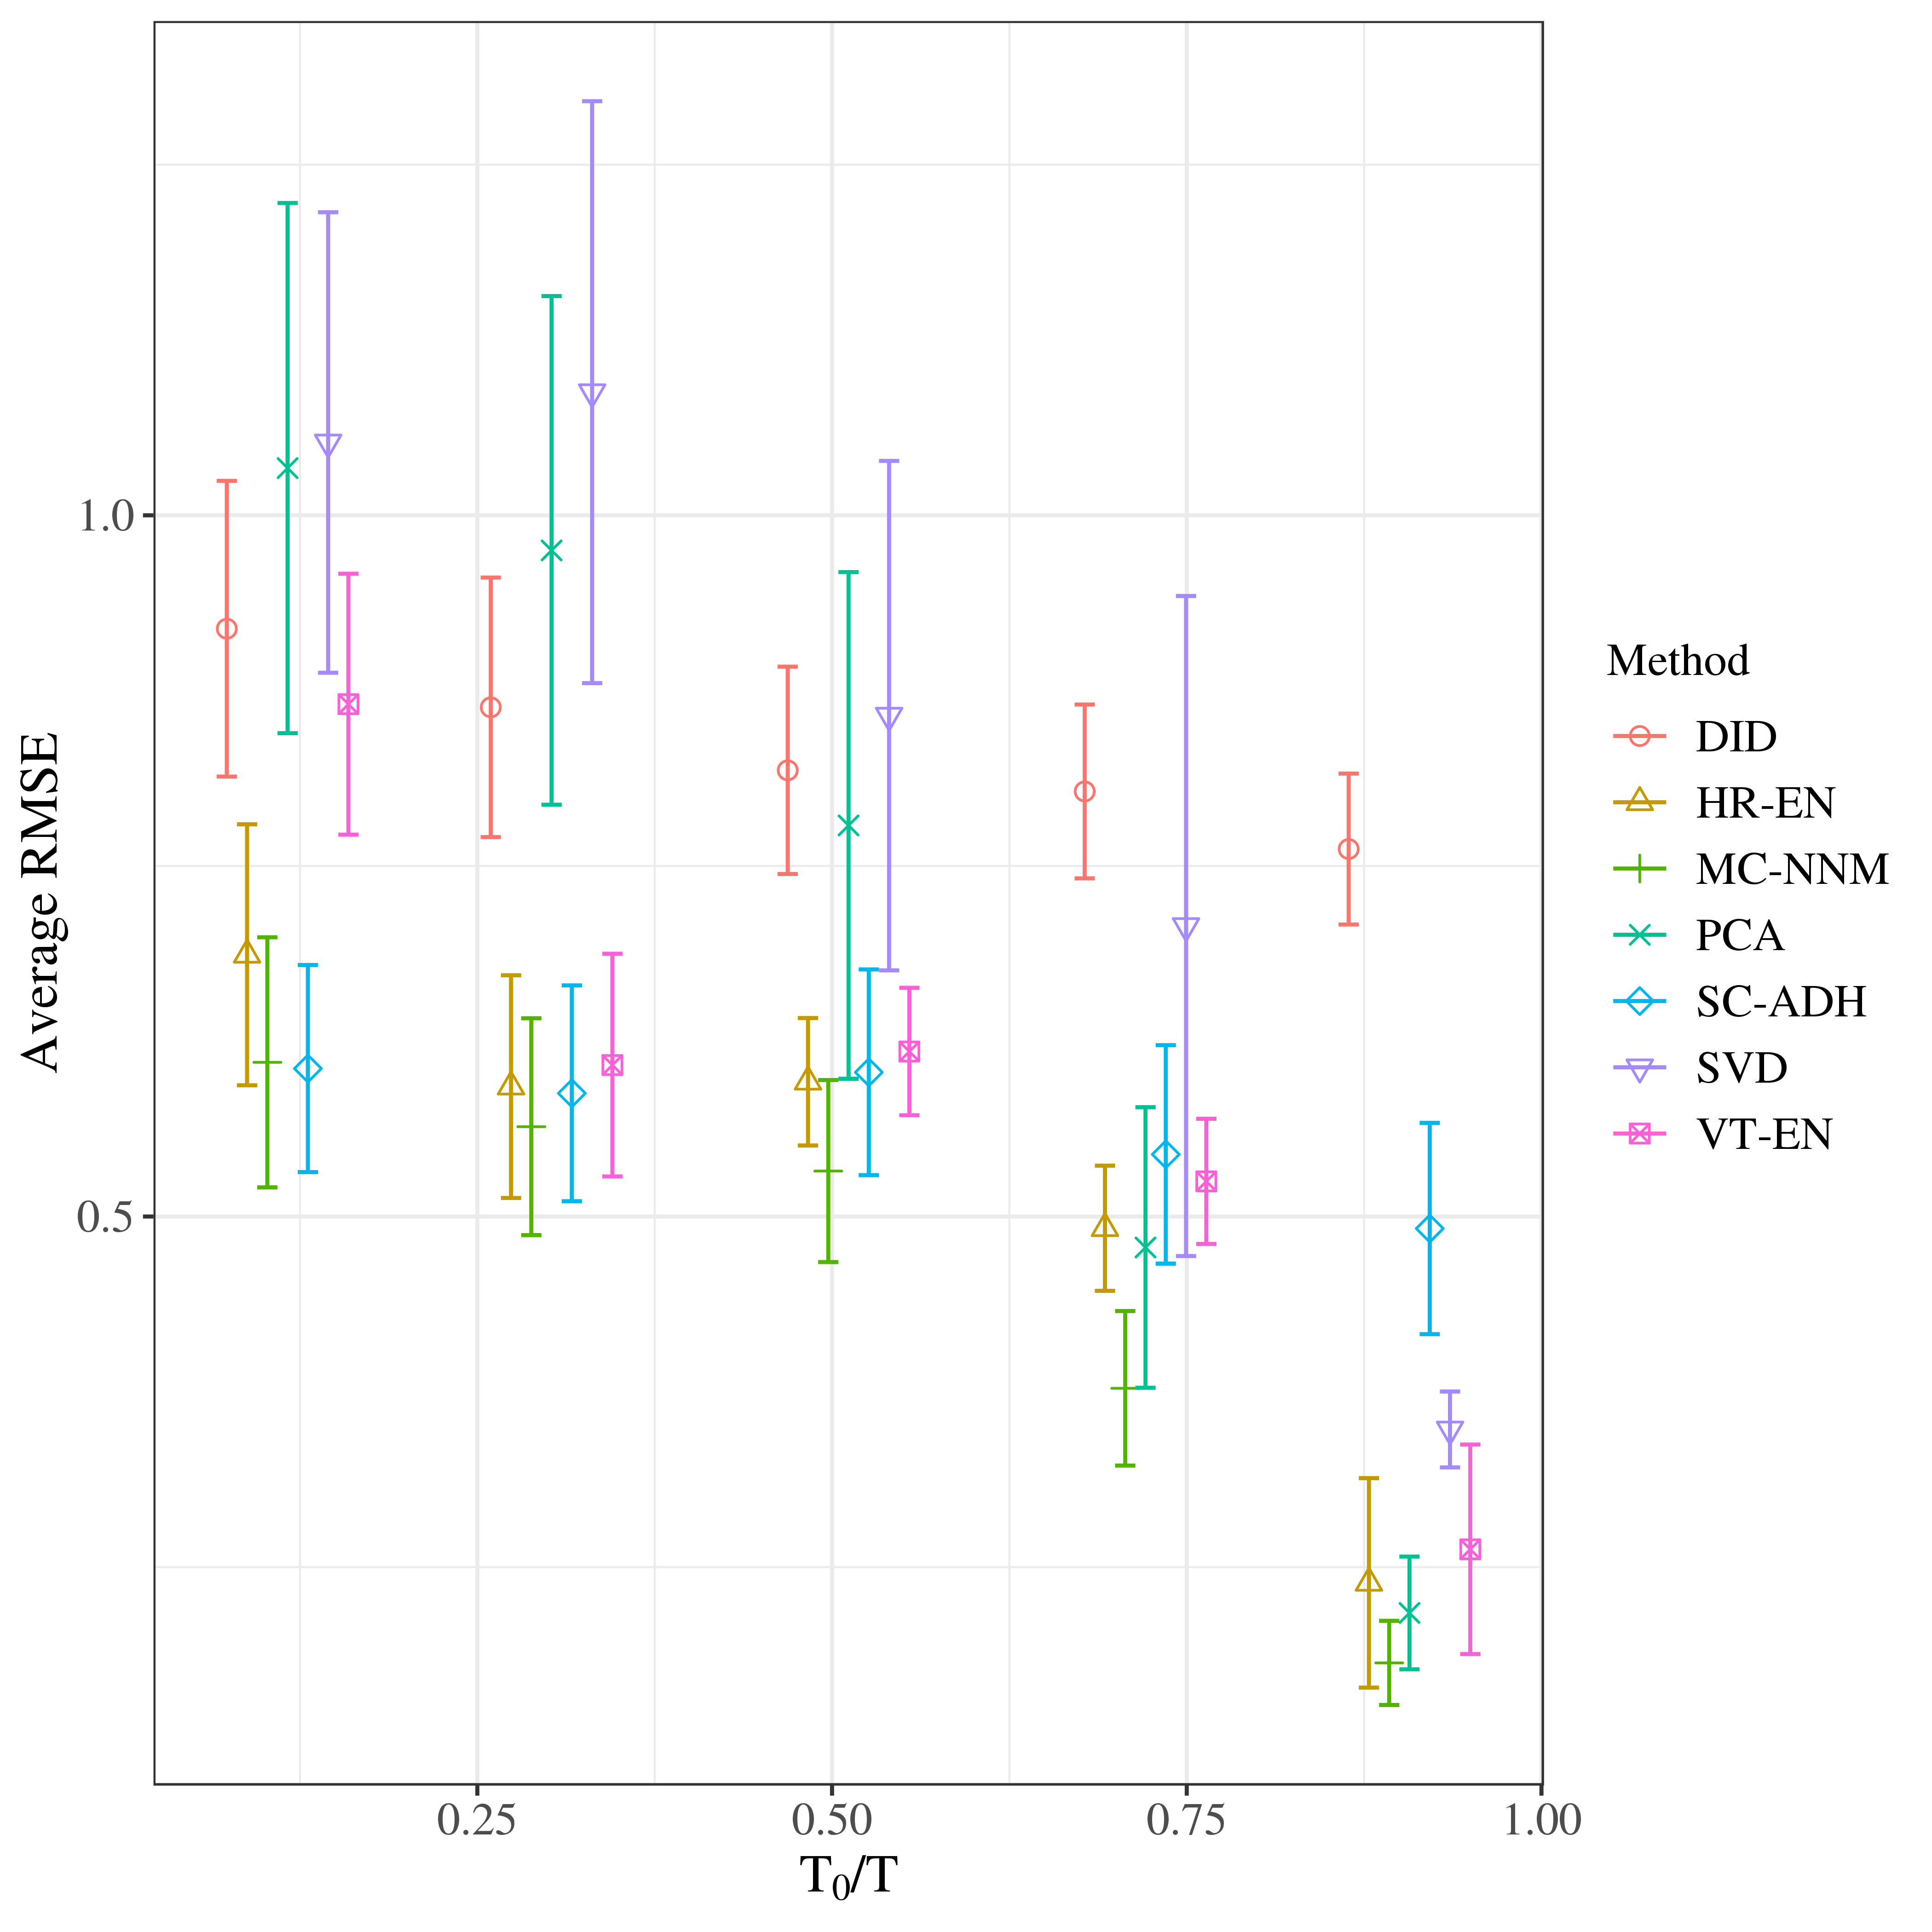
\includegraphics[width=\textwidth]{plots/basque_N_16_T_43_numruns_20_num_treated_8_simultaneuous_0.png}
		\caption{Basque Country terrorism data, $N_t = 8$} 
	\end{subfigure}
	~ 
	\begin{subfigure}[t]{0.48\textwidth}
		\centering
		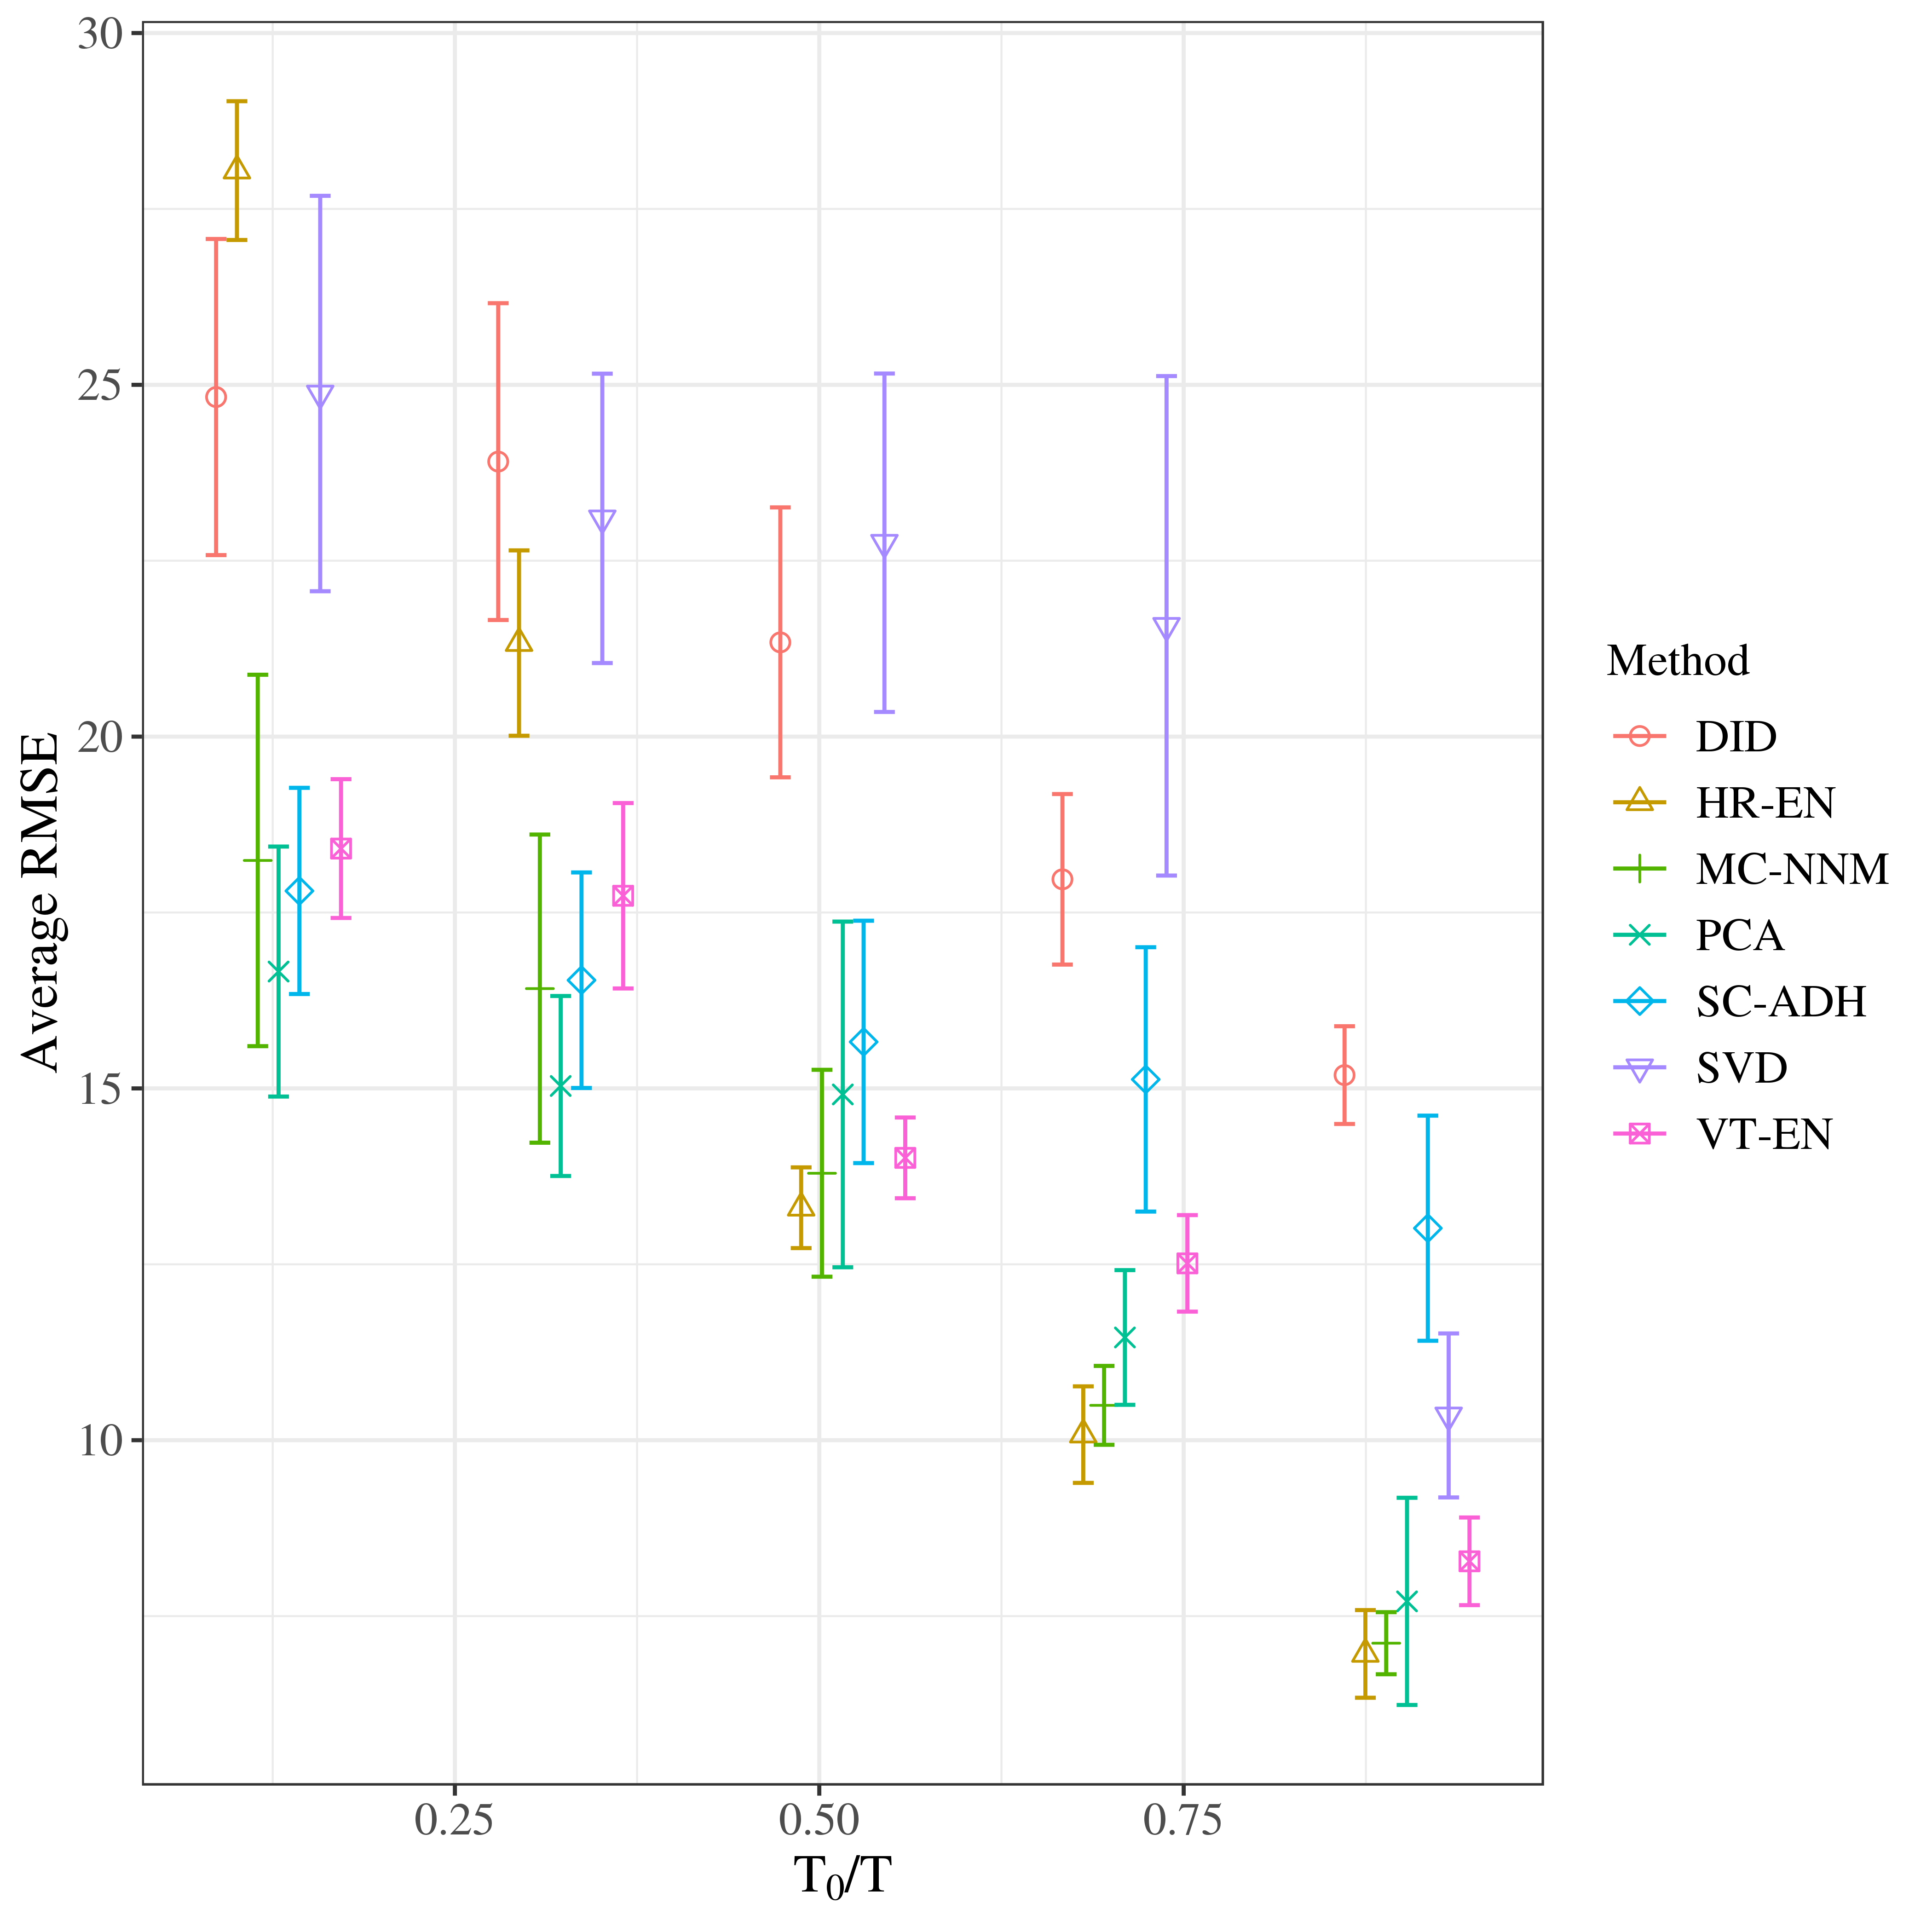
\includegraphics[width=\textwidth]{plots/california_N_38_T_31_numruns_20_num_treated_19_simultaneuous_0.png}
		\caption{California smoking ban data, $N_t = 19$}
	\end{subfigure}
	~ 
	\begin{subfigure}[t]{0.48\textwidth}
		\centering
		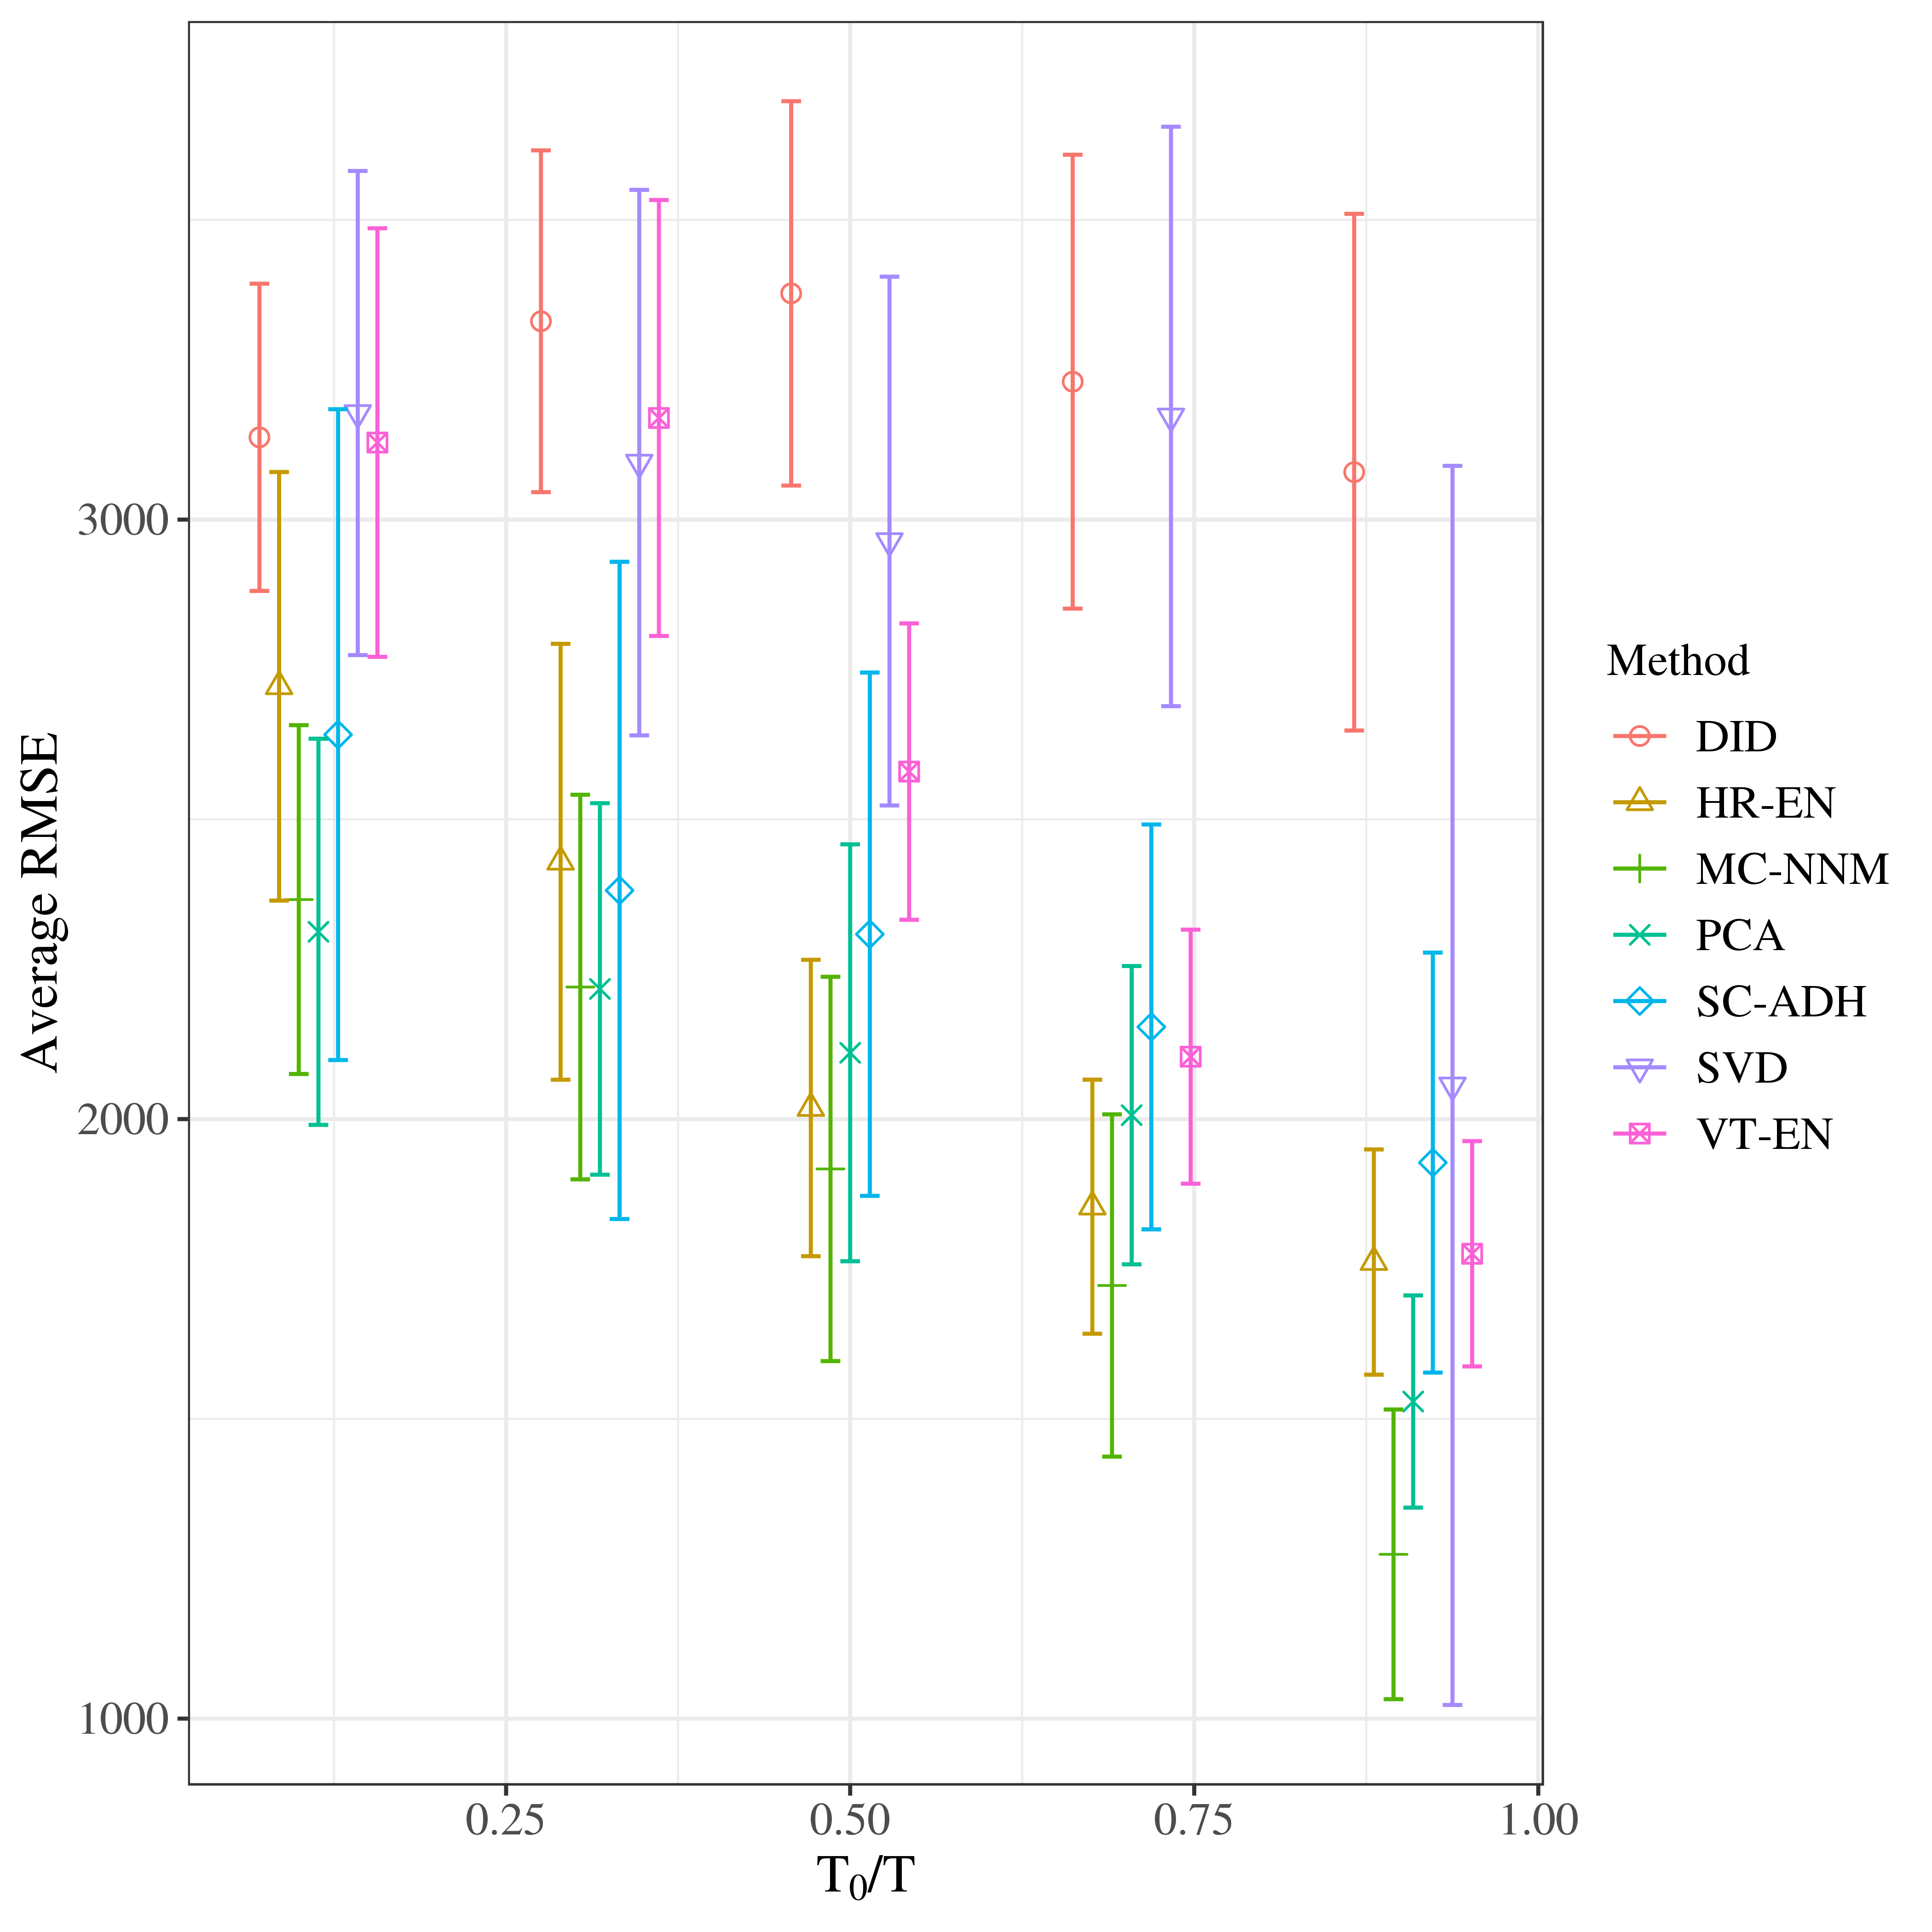
\includegraphics[width=\textwidth]{plots/germany_N_16_T_44_numruns_20_num_treated_8_simultaneuous_0.png}
		\caption{West German reunification data, $N_t = 8$}
	\end{subfigure}
	\caption{Placebo tests under staggered treatment adoption. Error bars represent 95\% confidence intervals calculated using the standard deviation of the prediction distribution for 20 trial runs. Note that the estimates are jittered horizontally to reduce overlap. \label{synth-stag}} 
\end{figure}

\subsection{Hypothesis testing} \label{hyp-test}

Consider a setup with $J$ control units indexed by $i=1, \ldots, J$ and $L$ treated units indexed by $i = J+1, \ldots, L+N$. The MC-NNM estimator imputes the missing post-period treated unit outcomes $\hat{Y}_{it} = \hat{L}_{it}$, for $J+1 \leq i \leq N$ and $T_0+1 \leq t \leq T$, where $T_0$ denotes the number of pre-periods. The inferred causal effect of the intervention on the treated group is the difference between the observed outcomes of the treated units and the counterfactual outcomes that would have been observed in the absence of the intervention:
%
\begin{align}
\hat{\alpha}_{it} &= Y_{it} - \hat{Y}_{it}, \hspace{10mm} J+1 \leq i \leq N, \, \hspace{5mm} \, T_0+1 \leq t \leq T \\ 
\hat{\bar{\alpha}}_{t} & = \frac{1}{L} \sum^{N}_{i=J+1} \hat{\alpha}_{it},  \label{eq:avg-pointwise}
\end{align}
%
where $\hat{\bar{\alpha}}_{t}$ corresponds to the per-period estimated average causal effect across treated units. 

\citet{chernozhukov2017exact} propose a randomization inference approach for testing the sharp null hypothesis $
\text{H}_0: \hat{\bar{\alpha}}_{t} = \bar{\alpha}^{o}_{t}$ for $T_0+1 \leq t \leq T,$
where $\left\{\bar{\alpha}^{o}_{t}\right\}_{t=T_0}^T$ is a trajectory of per-period average effects under the null. The test statistic suggested by \citet{chernozhukov2017exact} summarizes the trajectory of causal effects over the post-period:
%
\begin{equation} \label{tstat}
S (\hat{\bar{\alpha}}_{t}) = \left(\frac{1}{\sqrt{T_\star}} \sum_{t=T_0 +1}^{T} |\hat{\bar{\alpha}}_{t}|^q\right)^q,
\end{equation}
%
where $T_\star = T-T_0$ and $q \in \left\{1, 2\right\}$ in the applications. I estimate $p$-values by creating $\pi \in \Pi$ permutations of $\mathbf{Y}$ across the time dimension and calculating the proportion of test statics calculated on the permuted data under the null that are more extreme than the observed test statistic:
%
\begin{equation}
\hat{p} = \frac{1}{\Pi} \sum_{\pi \in \Pi} \textbf{1} \left\{S (\hat{\bar{\alpha}}_{\pi}) > S (\hat{\bar{\alpha}}_{t}) \right\}, \label{eq:pvalue}
\end{equation}
%
where $\hat{\bar{\alpha}}_{\pi}$ is the average causal effect estimated on the permuted data $\mathbf{Y_\pi}$. The idea for permuting time periods rather than treatment assignment is if the data are stationary and weakly dependent, which is often the case in an aggregate time-series setting, then the distribution of the error term $\epsilon$ in Equation (\ref{eq:mc-Y}) should be the same in the pre- and post-periods. \citet{chernozhukov2017exact} prove that the $p$-values resulting from their inferential procedure are approximately unbiased assuming that the MC-NNM estimator is consistent, which can be verified by placebo tests such as those described in Section \ref{placebo-tests}. I rely on three types of permutations: \emph{i.i.d.} random permutations of the time index $t$; \emph{i.i.d. block} random permutations of $K=T/b$ non-overlapping blocks, where $b$ is selected according to the optimal block length for the dependent bootstrap \citep{politis2004automatic}; and \emph{moving block} permutations that circularly shift $t$ by one period, resulting in $T-1$ permutations. The latter two permutations are capable of preserving the dependence structure of the data and are thus appropriate for weakly dependent data. 

\section{Impact of homestead acts on state capacity} \label{state-capacity}

Did homestead acts impact state capacity over the long-run? In this section, I estimate the causal impact of homestead acts on frontier state government finances. I use measures of total expenditure and revenue collected from the records of 48 state governments during the period of 1783 to 1932 \citep{sylla1993sources} and the records of 16 state governments during the period of 1933 to 1937 \citep{sylla1995sourcesa,sylla1995sourcesb}. Comparable measures for 48 states are drawn from U.S. Census special reports for the years 1902, 1913, 1932, 1942, 1962, 1972, and 1982 \citep{haines2010}.\footnote{I take the mean of duplicate state-year observations, which arise for the years 1902, 1913, and 1932.}% In order to capture a state's ability to fund public schooling, I create a measure of state government education spending from the state government expenditure sub-classifications. 

The outcomes data pre-processing steps are as follows. Each measure is inflation-adjusted according to the U.S. Consumer Price Index \citep{williamson2017seven} and scaled by the total free population in the decennial census \citep{haines2010}. I impute missing values separately in the pre- and -post-periods by carrying the last observation forward and impute remaining missing values by carrying the next observation backward. The raw outcomes data are log-transformed to alleviate exponential effects. Removing states with no variance in the pre-intervention outcomes results in complete $N \times T$ matrices of size $33 \times 159$ and $34 \times 158$, for the expenditures and revenues outcomes, respectively. 

The staggered adoption setting is appropriate for the current application because the year of initial treatment exposure $T_0$ varies across states, about half of which are exposed to homesteads following the passage of the HSA. I determine the years of initial exposure to homesteads by aggregating to the state level approximately 1.46 million individual land patent records authorized under the HSA. Land patent records provide information on the initial transfer of land titles from the federal government and are made accessible online by the U.S. General Land Office (\url{https://glorecords.blm.gov}). The earliest successful homestead filings occurred in 1869 in about half of the western frontier states, about seven years following the enactment of the HSA. The first homesteads were filed in southern states in 1872. Figure SM-\ref{fig:homestead-heatmap} visualizes the timing and intensity of homestead entries. 

Unit-specific covariates $\mathbf{X}$ include state-level average farm sizes measured in the 1860 and average farm values measured in the 1850 and 1860 censuses.\footnote{Table SM-\ref{dv-table} provides data sources and definitions.} In theory, we should expect that homesteaders migrate to more productive land and thus excluding these pre-intervention measures of agricultural productivity may result in overestimating the actual impact of homestead policy. To control for selection biases in terms of access to frontier lands, I create a measure of railroad access using digitized railroad maps provided by \citet{atack2013use}, which contain information on the year that each rail line was built. Overlaying the railroad track map over historical county borders, I calculate the total miles of operational track per square mile and aggregate the measure to the state-level.\footnote{Using these data, I estimate that 29\% of counties had railroad access in 1862 and 91\% had access by 1911 (Fig. SM-\ref{rr-map}). The railroad access measure defines access with respect to county boundaries, which \citet{atack2012impact} point out has limitations because a county without access might be adjacent to one with access and county boundaries frequently changed over time.}

\subsection{Placebo tests} \label{placebo-tests}

Prior to presenting the main results, I assess the validity of the key assumption underlying the approach by discarding post-period observations from the data and testing the null hypothesis 

\begin{equation} \label{h0-placebo}
\text{H}_0: S (\hat{\bar{\alpha}}_{t}) = 0  \, \hspace{5mm} \,  \text{for} \, \hspace{2mm} T_0 - \tau +1 \leq t \leq T_0,
\end{equation}
%\frac{1}{\tau +1} \sum_{T_0 - \tau +1}^{T_0} \hat{\bar{\alpha}}_{t} 
where $\tau \in \left\{1, 10, 25\right\}$. This placebo null hypothesis is tested by the same procedure described in Section \ref{hyp-test}, treating $\left\{1, \ldots, T_0 - \tau\right\}$ as the pre-period.

Table \ref{placebo-tests} reports the average treatment effect over the placebo post-period and randomization $p$-values calculated by Equation (\ref{eq:pvalue}). Placebo tests on the revenue outcome yield two-sided $p$-values greater than the significance level of $\alpha = 0.05$, regardless of the value of $q$ or permutation structure. These results provide evidence in favor of the validity of the consistency assumption. However, we can only reject the null in the case of $\tau=1$ when considering the expenditure outcome, which suggests that the consistency may only hold when the ratio $T_0/T$ is very high. 

\begin{table}[htbp]
	\captionsetup{font=normalsize}
	\caption{Placebo test $p$-values.\label{placebo-tests}}
	\begin{center}
		\scalebox{.95}{\begin{tabular}{@{}lccccccccc@{}}
		\toprule
		 & \multicolumn{3}{c}{Education Spending}        & \multicolumn{3}{c}{Expenditure}            & \multicolumn{3}{c}{Revenue}                \\ \midrule
		& $\tau = 10$   & $\tau = 20$   & $\tau = 30$   & $\tau = 10$  & $\tau = 20$  & $\tau = 30$  & $\tau = 10$  & $\tau = 20$  & $\tau = 30$  \\
		\hline
		Mean Effect                          & -0.43         & -0.34         & -0.26         & 0.1          & 0.05         & 0.02         & 0.05         & 0.03         & 0.03         \\
		i.i.d. Block CIs                       & [-1.45, 1.45] & [-1.07, 1.11] & [-0.62, 0.67] & [0.00, 0.00] & [0.00, 0.00] & [0.00, 0.00] & [0.00, 0.00] & [0.00, 0.00] & [0.00, 0.00] \\
		Moving Block CIs                       & [-1.16, 1.23] & [-0.95, 0.92] & [-0.62, 0.69] & [0.00, 0.00] & [0.00, 0.00] & [0.00, 0.00] & [0.00, 0.00] & [0.00, 0.00] & [0.00, 0.00] \\ \bottomrule
\end{tabular}
}
	\end{center}
	\footnotesize{\emph{Notes:} randomization $p$-values corresponding to each permutation structure and value of $\tau$ and $q$. i.i.d. block and i.i.d. block $p$-values are calculated using $|\Pi| = 1,000$ permutations. Moving block $p$-values are based on $|\Pi| = T-1$ permutations.}
\end{table}

Further evidence of the consistency of the MC-NNM estimator is provided in Figure SM-\ref{mc-sim}, which presents the results of placebo tests on control units using both pre- and post-period observations for each outcome. Similar to the simulations on the SCM datasets discussed in Section \ref{sims}, there are no missing entries in each outcome $\mathbf{Y}$ because the actual treated units are removed prior to the placebo tests. I randomly choose about half of the remaining control units as hypothetical treated units and predict their values for time periods following a randomly selected $T_0$. 

The MC-NNM estimator outperforms DID and SVD estimators in terms of minimizing RMSE for each ratio $T_0/T$. At $T_0/T \geq 0.5$, the estimator generally yields comparable error rates to PCA, SCM, and vertical regression estimators. 

\subsection{Main estimates}

In the main analyses, I fit the MC-NNM estimator described in Equation \ref{eq:mc-Y} on the entirety of observed entries in $\mathbf{Y}$ to recover its missing entries; i.e., the counterfactual outcomes of public land states. The value of the regularization term $\lambda$ is optimally selected on the value that yields the lowest average RMSE calculated during cross-validation. The average RMSE calculated on the validation sets during the $\lambda$ selection process are 0.41 and 0.48 for the expenditures and revenues outcomes, respectively. 

The top panels of Figure \ref{mc-estimates-exp-pc} and \ref{mc-estimates-rev-pc} compare the means of the observed time-series of treated units and control units along with the mean predicted outcomes of treated units. The observed means of the treated and control units are essentially identical in the post-period. However, we are interested primarily in the difference in the observed and predicted treated unit outcomes, which is the quantity $\hat{\bar{\alpha}}_{t}$ in Equation (\ref{eq:avg-pointwise}). This quantity corresponds to the estimated per-period average causal effects of treatment exposure on the treated units and the per-period effects are plotted in the bottom panels. For display purposes, bootstrap confidence intervals for $\hat{\bar{\alpha}}_{t}$ are calculated by block resampling with optimal block lengths selected by the procedure described by \citet{politis2004automatic}. 

Table \ref{mc-estimates} reports randomization $p$-values from testing the null hypothesis of a zero effect:

\begin{equation} \label{h0}
\text{H}_0: S (\hat{\bar{\alpha}}_{t}) = 0  \, \hspace{5mm} \,  \text{for} \, \hspace{2mm} T_0 + 1 \leq t \leq T.
\end{equation}

\begin{figure}[htbp]
	\centering
%	\begin{subfigure}[t]{0.48\textwidth}
%		\centering
%		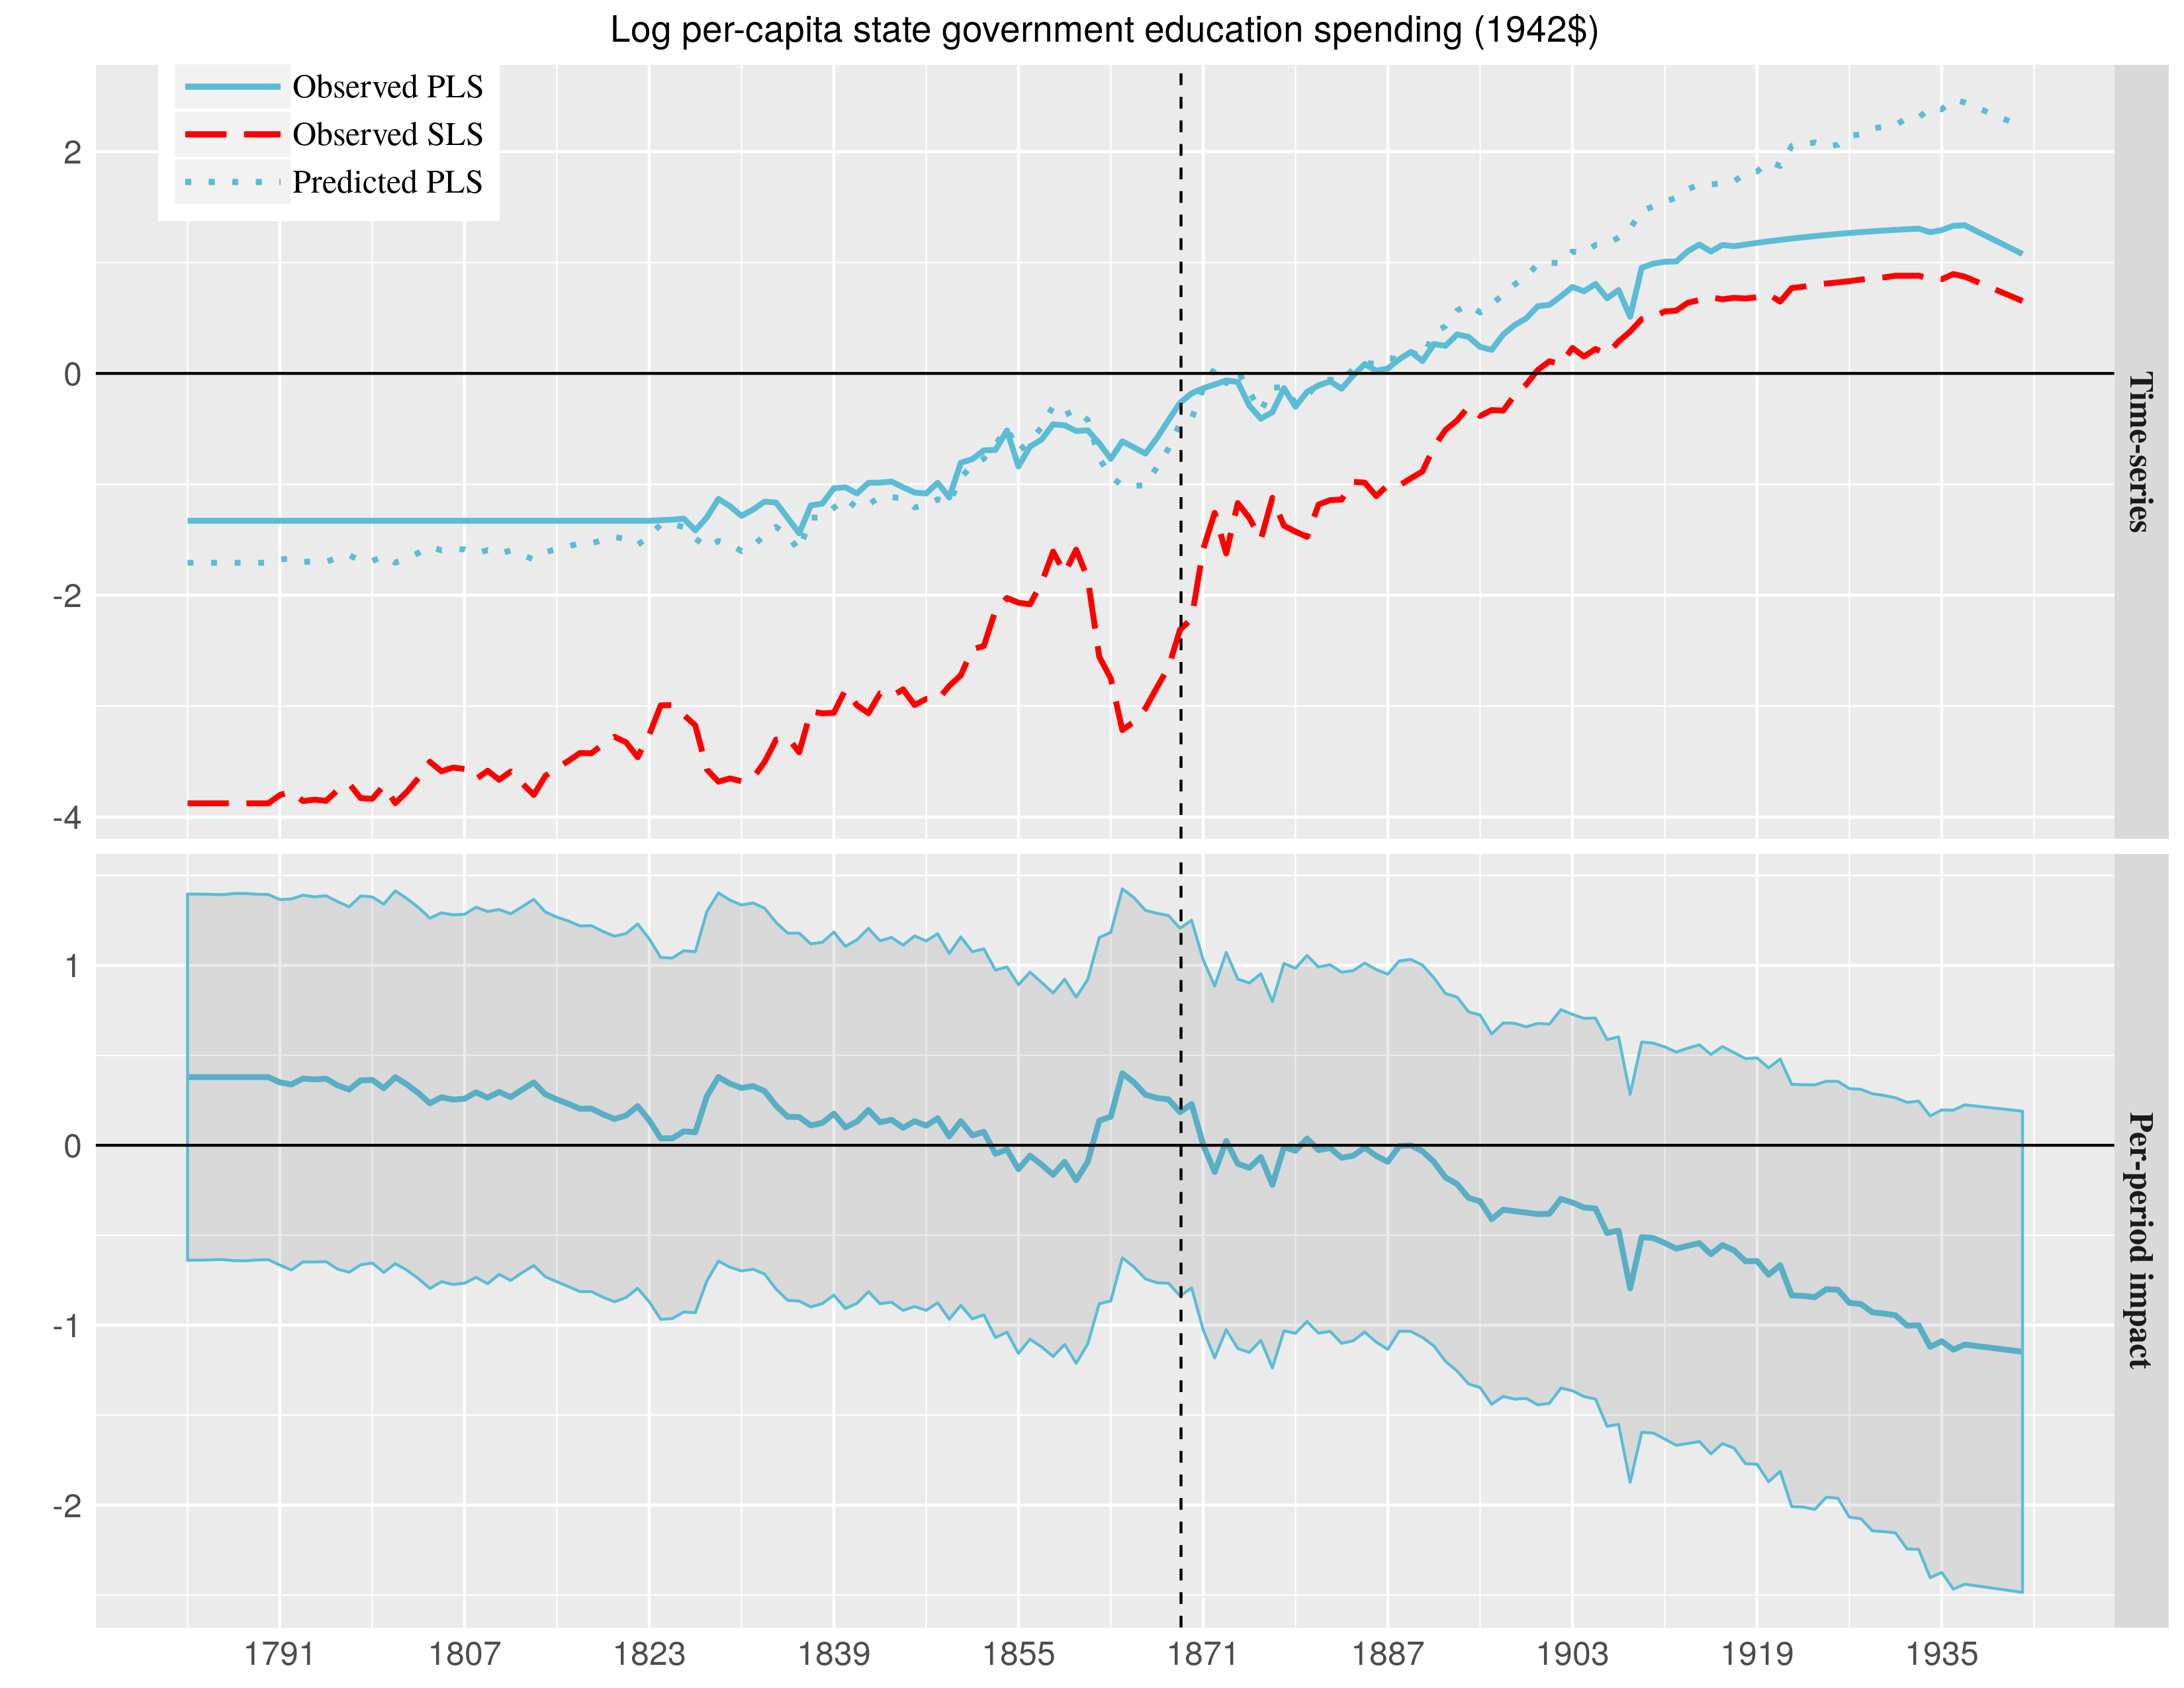
\includegraphics[width=\textwidth]{plots/mc-educ-pc.png}
%		\caption{State government education spending}
%	\end{subfigure}
%	~ 
	\begin{subfigure}[t]{0.75\textwidth}
		\centering
		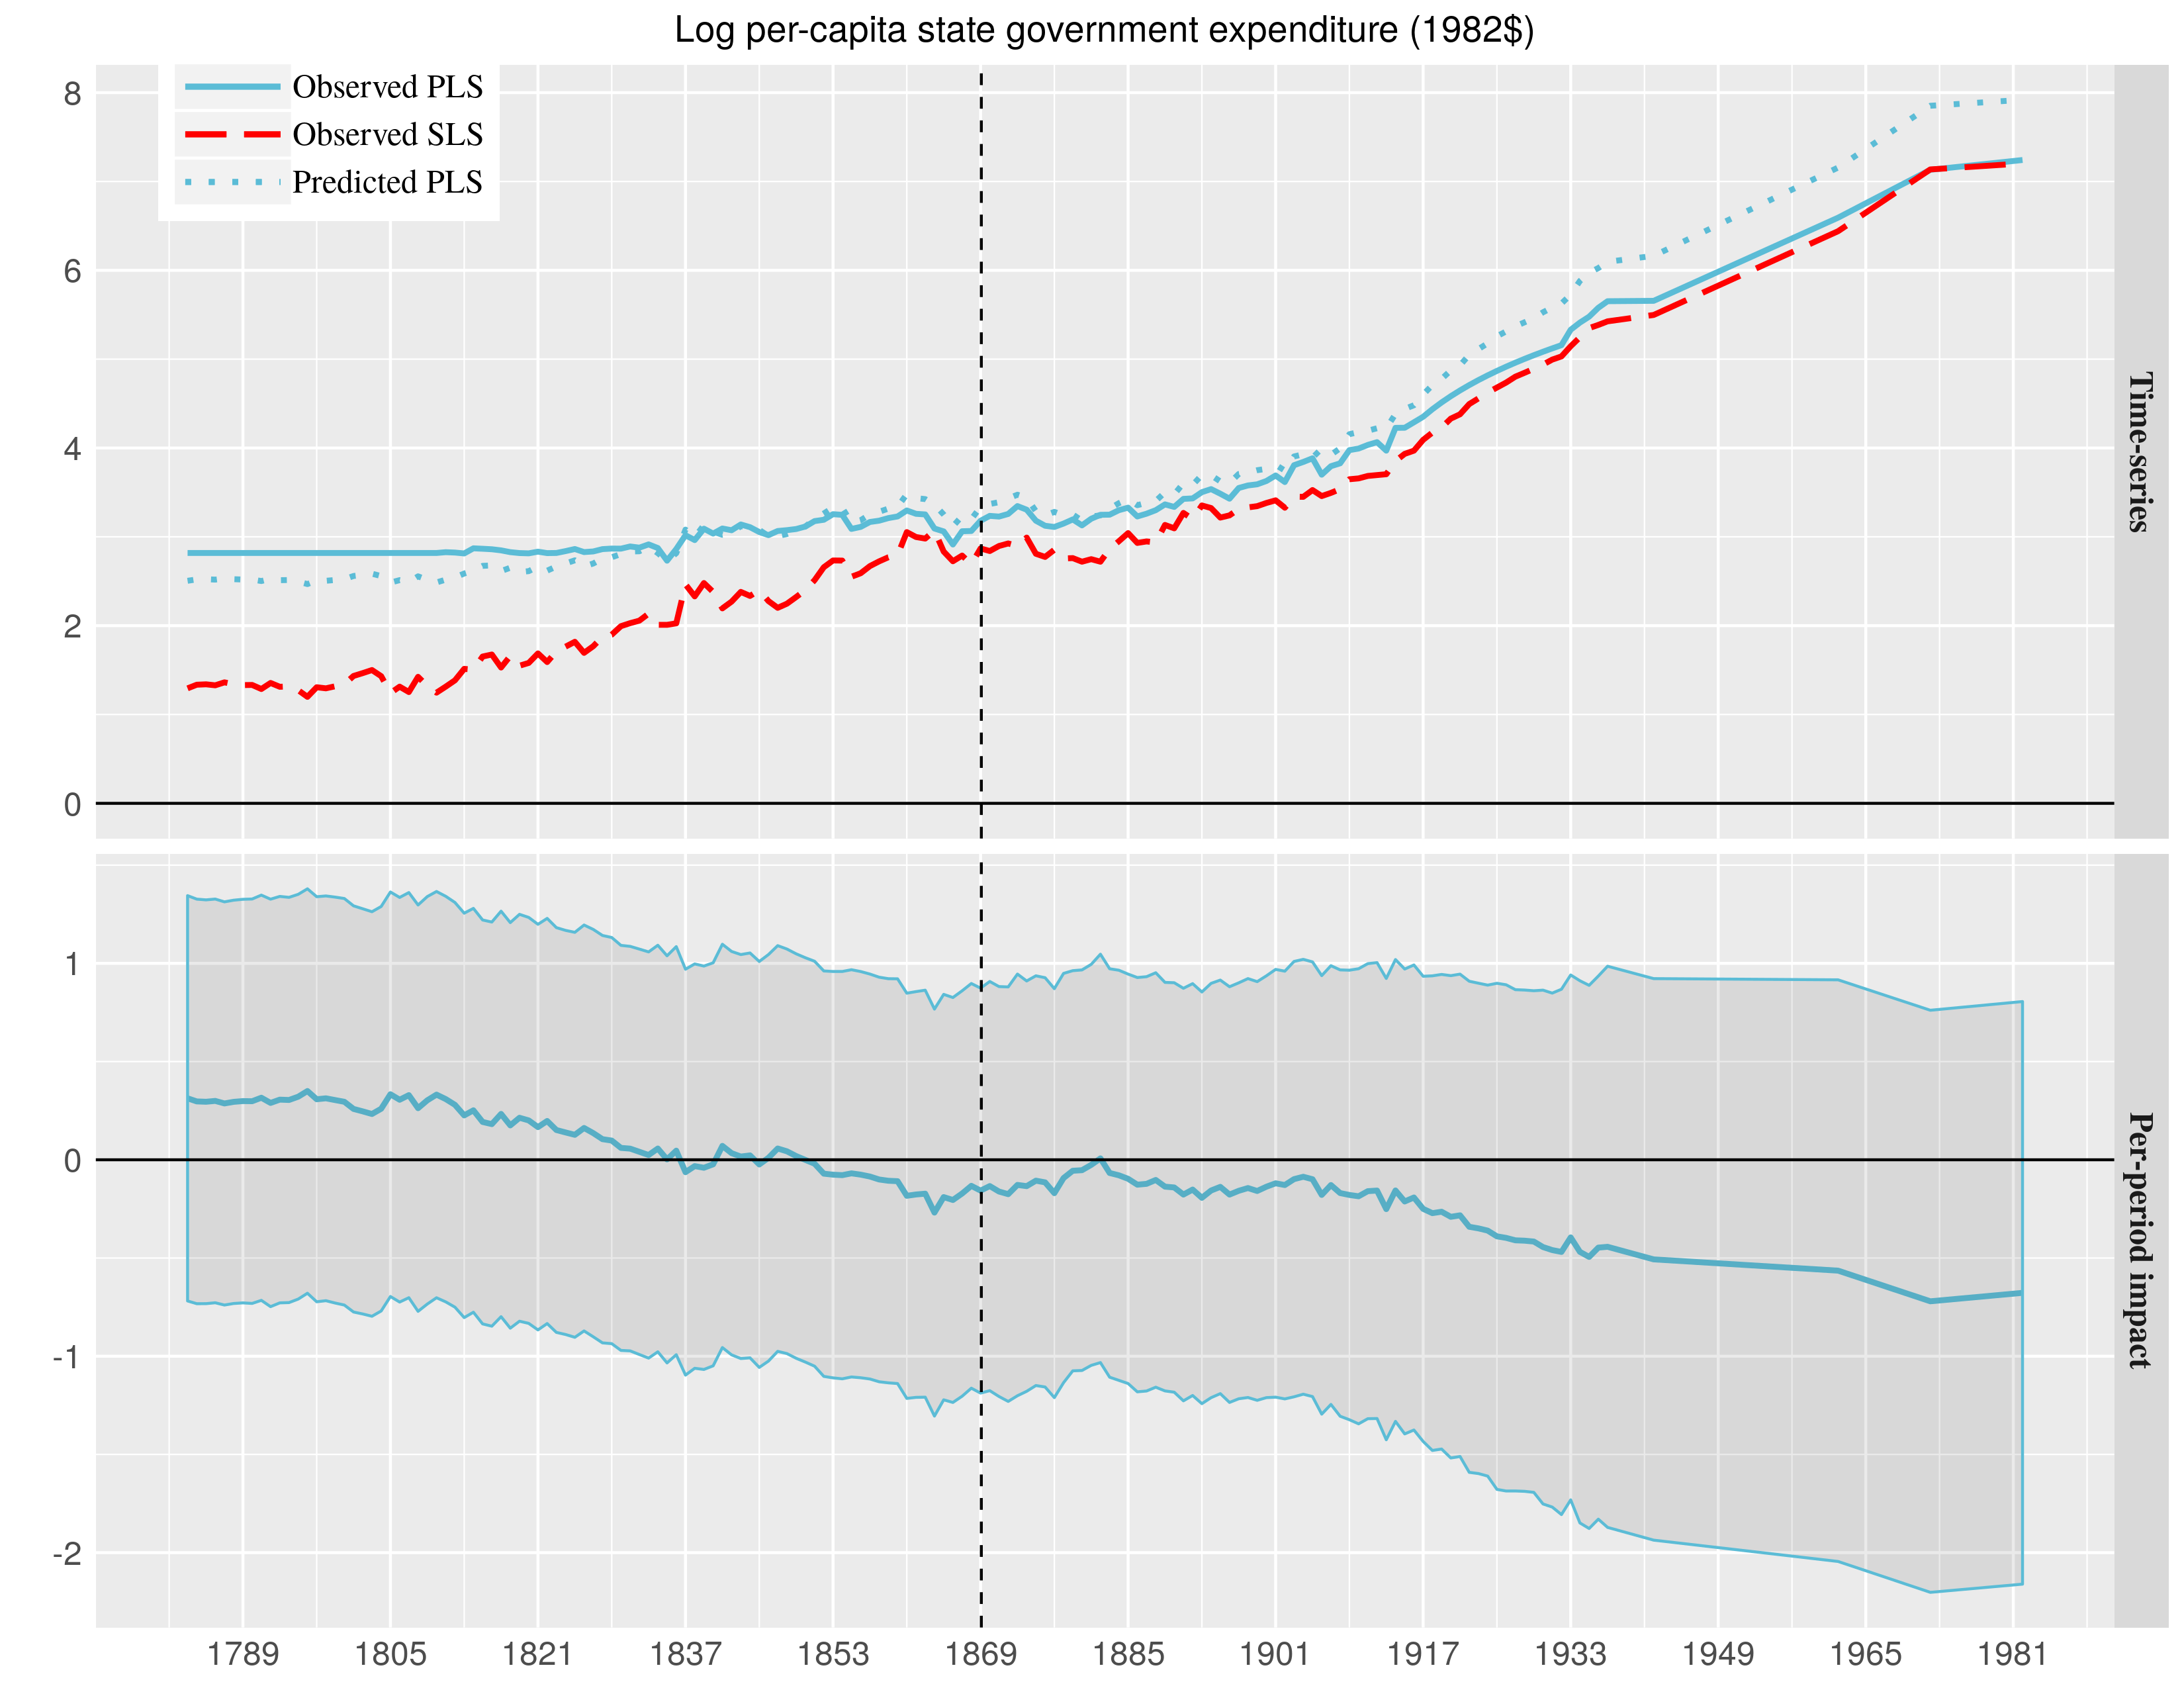
\includegraphics[width=\textwidth]{plots/mc-exp-pc.png}
		\caption{Log per-capita state government expenditure (1982\$)\label{mc-estimates-exp-pc}}
	\end{subfigure}
	~ 
	\begin{subfigure}[t]{0.75\textwidth}
		\centering
		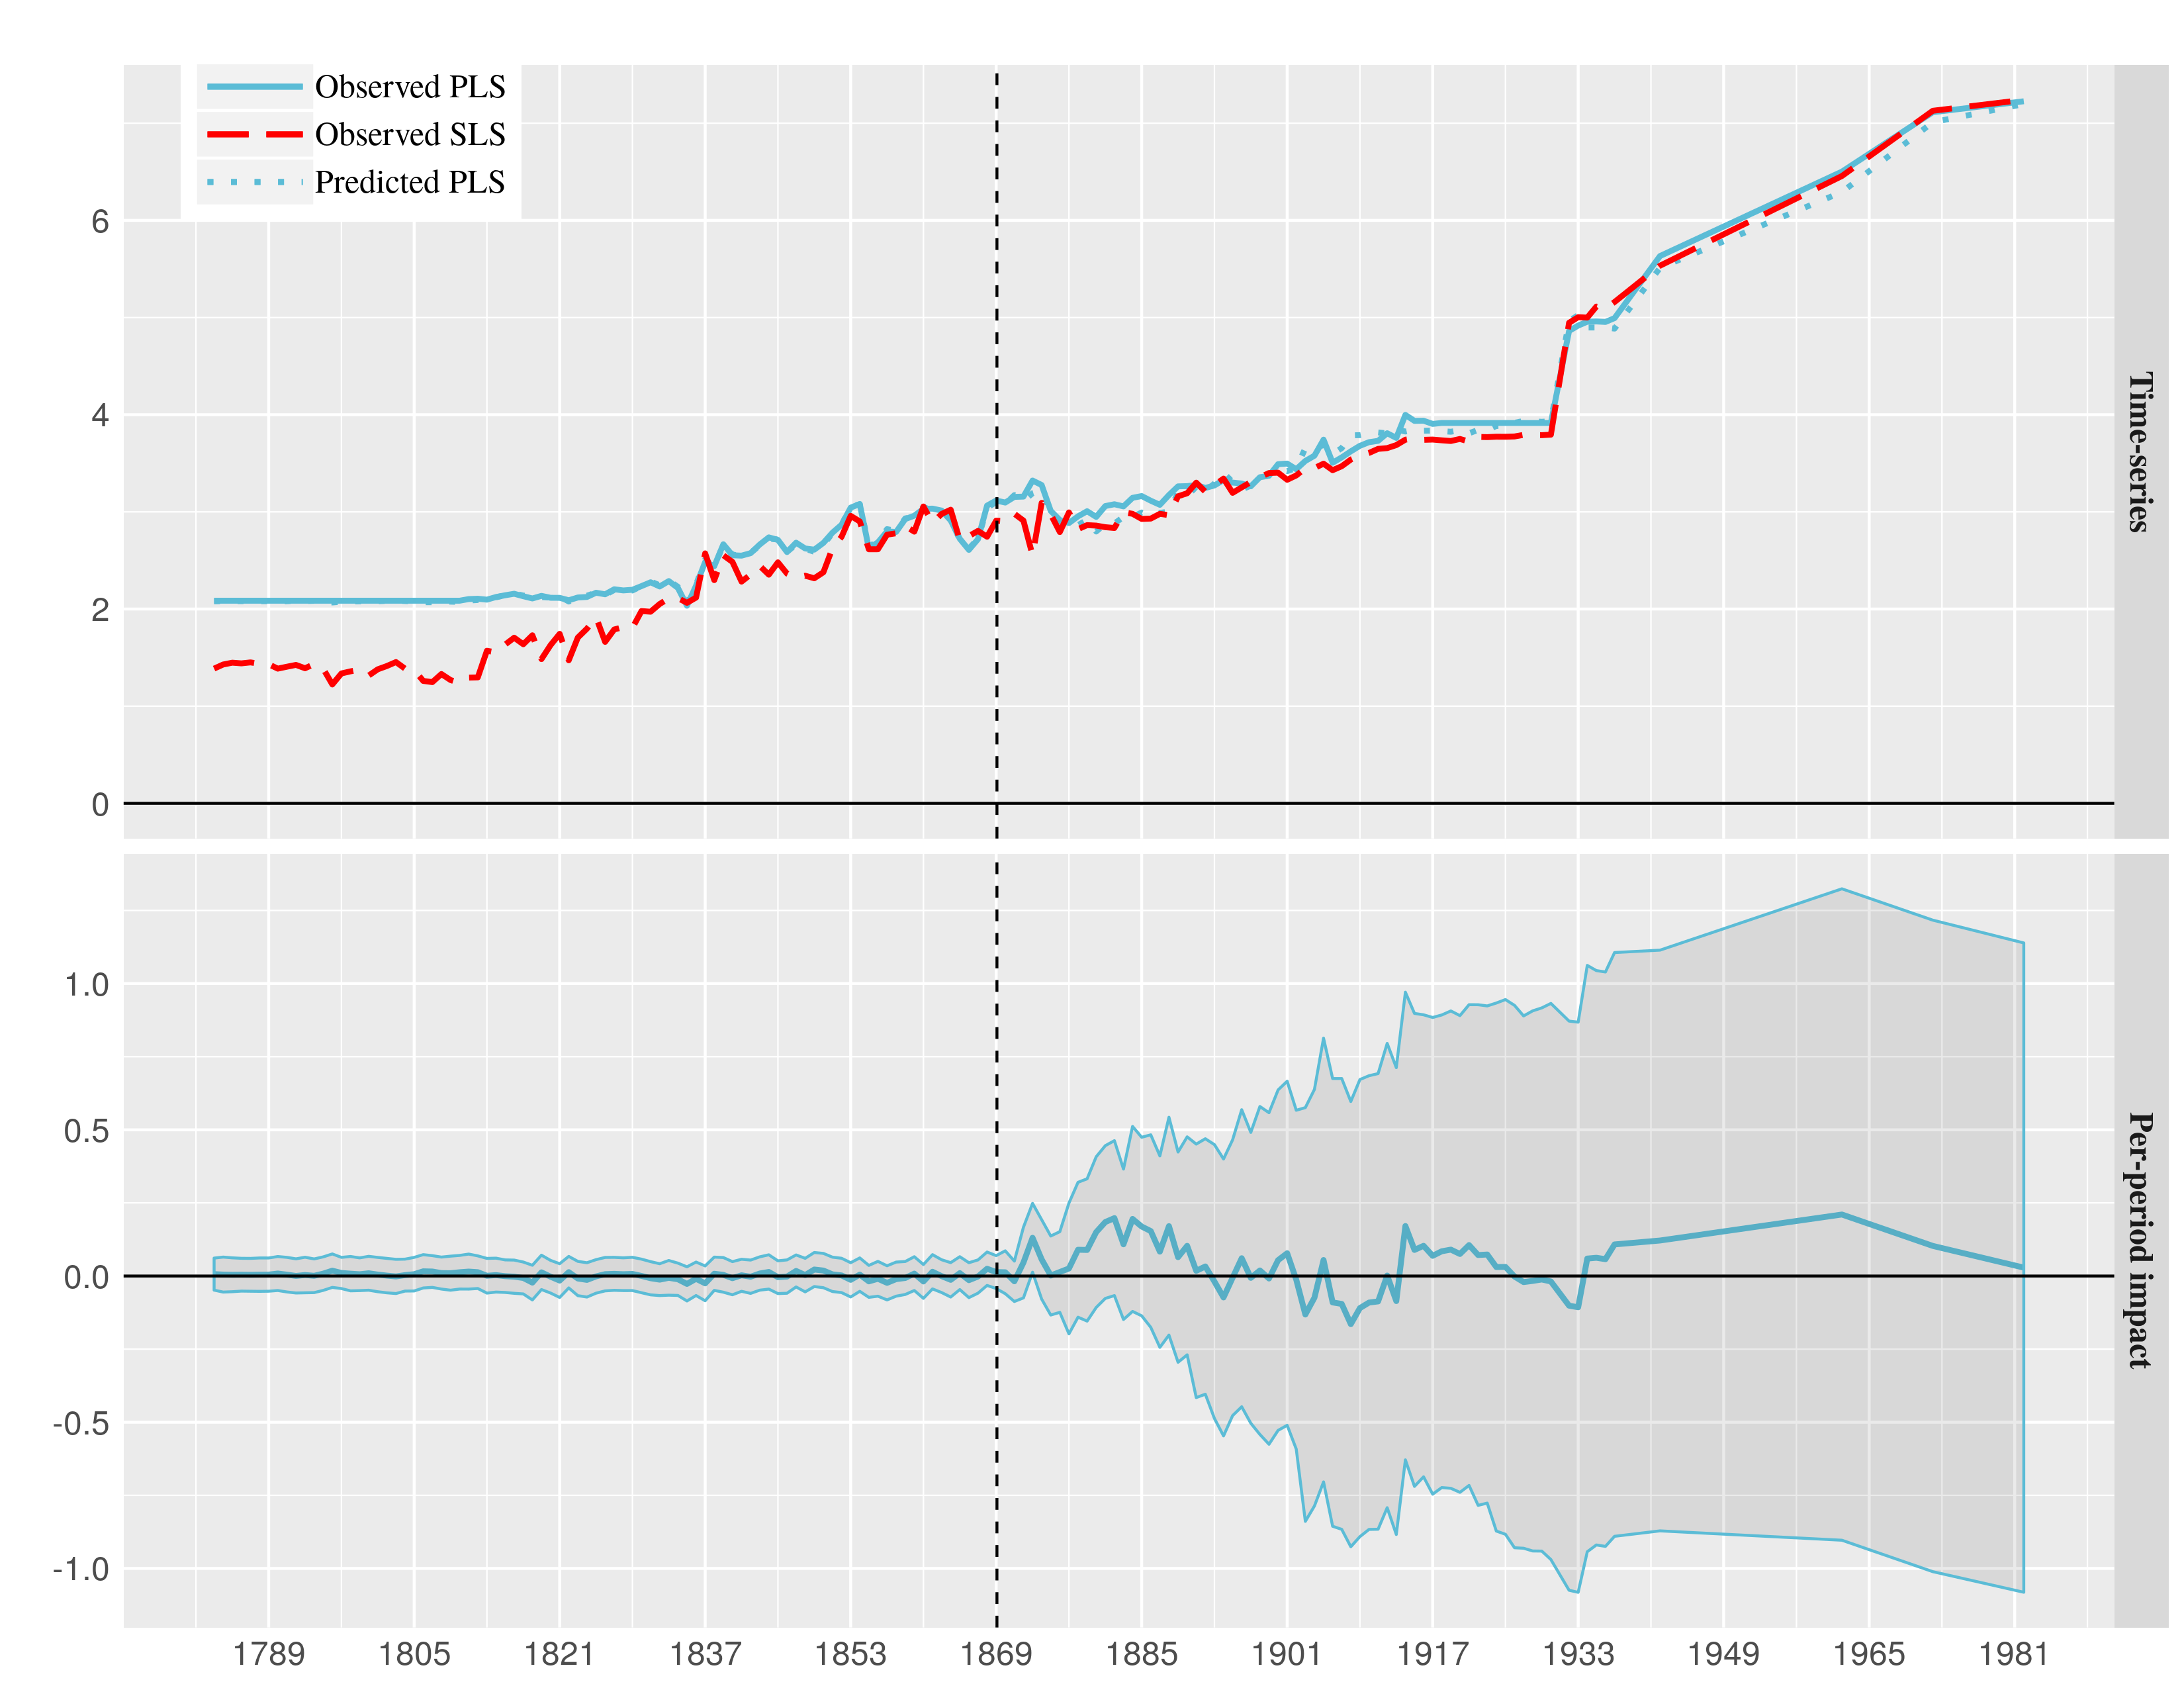
\includegraphics[width=\textwidth]{plots/mc-rev-pc.png}
		\caption{Log per-capita state government revenue (1982\$)\label{mc-estimates-rev-pc}}
	\end{subfigure}
	\caption{Top panel: Mean observed (solid time-series) and counterfactual predicted (dotted time-series) outcomes of treated units (PLS) and mean observed outcomes (dashed time-series) among control units (SLS), displayed for the time period of 1809 to 1982. Dashed vertical line represents the initial treatment year of 1869. Bottom panel: Per-period average causal impacts of homestead exposure on PLS, or $\hat{\bar{\alpha}}_{t}$ in Equation (\ref{eq:avg-pointwise}). Shaded regions represent 95\% confidence intervals estimated by taking $\hat{\bar{\alpha}}_{t} \pm 1.96$ the standard error of the distribution of 1,000 bootstrap replicates of $\hat{\bar{\alpha}}_{t}$.\label{mc-estimates}} 
\end{figure}


\begin{table}[htbp]
	\captionsetup{font=normalsize}
	\caption{Causal estimates on state capacity datasets.\label{mc-estimates}}
	\begin{center}
		%\begin{tabular}{@{}lcc@{}}
%	\toprule 
%	& \multicolumn{2}{c}{ Education Spending } \\
%\hline
%	& $q=1$ & $q=2$ \\
%\hline \\
%	$S (\hat{\bar{\alpha}}_{t})$ & 3.81 & 1.66 \vspace{2mm}\\
%	i.i.d. & 0 & 0 \\
%	i.i.d. Block & 0.02 & $<0.01$3 \\
%	Moving Block & 0.23 & 0 \\
%		 &  &  \\
%	& \multicolumn{2}{c}{ Expenditure }\\
%\hline
%	& $q=1$ & $q=2$ \\
%\hline \\
%	$S (\hat{\bar{\alpha}}_{t})$ & 1.99 & 0.81\vspace{2mm} \\
%	i.i.d. & 0.39 & 0.49 \\
%	i.i.d. Block & 0.50 & 0.49 \\
%	Moving Block & 0.41 & 0.38 \\
%			 &  &  \\
%	& \multicolumn{2}{c}{ Revenue }\\
%\hline
%	& $q=1$ & $q=2$ \\
%\hline \\
%	$S (\hat{\bar{\alpha}}_{t})$ & 1.28 & 0.62\vspace{2mm} \\
%	i.i.d. & 0.99 & 0.85 \\
%	i.i.d. Block & 0.89 & 0.64 \\
%	Moving Block & 0.74 & 0.41 \\
%\bottomrule
%\end{tabular}
\begin{tabular}{@{}lcccc@{}}
	\toprule 
	& \multicolumn{2}{c}{ Expenditure } & \multicolumn{2}{c}{ Revenue } \\
	\hline
	& $q=1$ & $q=2$ & $q=1$ & $q=2$ \\
	\hline \\
	$\text{S}_q (\boldsymbol{\hat{\bar{\upalpha}}})$ & 3.87 & 1.40 & 1.97 & 0.76\vspace{2mm}\\
	i.i.d. & 0.002 & 0.003 & 0.001 & 0.001\\
	i.i.d. Block & 0.001 & 0.002 & 0.001 & 0.001\\
	Moving Block & $<0.001$ & $<0.001$ & $<0.001$ & $<0.001$ \\
	\bottomrule
\end{tabular}

	\end{center}
	\footnotesize{\emph{Notes:} $S (\hat{\bar{\alpha}}_{t})$ corresponds to the test statistic described in Equation (\ref{tstat}) and each value beneath is the randomization $p$-value corresponding to each permutation structure. See footnotes to Table \ref{placebo-tests}.}
\end{table}

\section{DID estimation} \label{DID}

The matrix completion approach estimates the impact of a discrete event on a continuous outcome. However, in this application a continuous form of treatment is available in the form of homestead entries. Equation (\ref{eq:dd}) estimates a continuous version of the DID estimator described in Section \ref{sims}. Similar to the case of binary treatment, the continuous DID estimator is adapted to a setting of staggered adoption because the initial date of exposure to homesteads varies across public land states. The first difference comes from variation in the date of initial exposure to homesteads, and the second difference comes from variation in the intensity of homestead entries.
%
\begin{equation} %check Acemoglu model
Y_{i, t} =  a_i + b_t + \gamma \, M_{it} + \delta \, (M_{it} \cdot \text{homesteads}_{it}) + X'_{it}  + \epsilon_{it}. \label{eq:dd} 
\end{equation}

In this model, $a_i$ and $b_t$ are vectors of unit and time fixed effects, respectively, included to control for unobserved heterogeneity across units. In the staggered adoption setting, entries in the missing value indicator $M_{it}$ assume the value of 1 at $t \geq T_0$, where the initial exposure time $T_0$ varies across units. The continuous treatment exposure variable $\text{homesteads}_{i, t}$ measures the per-capita statewide sum of homestead entries in state $i$ and year $t$.

The coefficient corresponding to the interaction term, $\hat{\delta}$, is the estimated average causal effect of exposure to homesteads. I use unit-stratified bootstrapped samples to construct nonparametric standard errors for $\hat{\delta}$.\footnote{The model assumes i.i.d. errors, which understates the standard errors for $\hat{\delta}$ when the regression errors are serially correlated, or $\mathrm{Corr} (\epsilon_{s, t}, \epsilon_{s, t-1}) \neq 0$, which can arise when the time-series lengths are not sufficiently long to reliably estimate the data generating process. \citet{bertrand2004much} show that the stratified bootstrap can be used to compute consistent standard errors when the number of units is sufficiently large.} $X'_{i,1860}$ is the average value of farm land in 1860, which is included to ensure that $\hat{\delta}$ is not biased by parallel trends in pre-intervention agricultural productivity. 

It should be emphasized that the DID estimator in a staggered adoption setting relies on several strong assumptions regarding both the assignment mechanism, which in this application is the distribution of initial treatment times $T_0$, and the counterfactual outcomes of the treated units. The framework of \citet{athey2018design}, for instance, assumes the distribution of $T_0$ is completely random conditional on $X'_{i,1860}$. In the current application, this assumption ignores the possibility that initial exposure to homesteads might be determined by unobserved factors. The framework also that the counterfactual outcomes at time $t$ does not depend on the future date of treatment exposure if $t < T_0$ or the history of treatment exposure if $t > T_0$. Violations of these assumptions would arise if the homestead policy is anticipated prior to $T_0$ or if the size of frontier state government is determined by whether the state was exposed early or late to homesteads. 

\subsection{DID estimates}
I apply the DID estimator on two unbalanced state-year panel datasets: the panel of southern public land states spans  from 1823 to 1982 and has 38 observations prior to the enactment of the SHA. The panel of western public land states spans from 1810 to 1982 and has 52 pre-intervention years. The treatment effect estimates, summarized in Fig.~\ref{fig:did-state-robust}, indicate that per-capita cumulative homesteads significantly increase per-capita revenue in western states by 0.02 log points [0.0007, 0.04] and has a nonsignificant impact on revenue in southern states. Estimates on per-capita expenditure in the South and West are also nonsignificant. Per-capita cumulative homesteads significantly raise education spending in the South by 0.17 log points [0.03, 0.28], while having no impact on education spending in the West. As expected, withholding average farm values from the DID specification biases treatment effect estimates upwards (Fig.~SM-\ref{fig:did-state-robust}).

\begin{figure}[htbp]
	\begin{center}
		\includegraphics[width=\textwidth]{/media/jason/Dropbox/github/land-reform/results/plots/did-state-robust.png}
	\end{center}
	\caption{DID estimates of log per-capita cumulative homesteads on log per-capita state government finances. Lines represent 95\% confidence intervals are constructed using 10,000 state-stratified bootstrap samples. Lines with triangles represent western public land state estimates and lines with circles represent southern public land state estimates.  \label{fig:did-state-robust}}
\end{figure}

%+Farm values *cumulative*
%south-educpc: 0.17 [0.03, 0.28]
%south-exppc: 0.03 [-0.03, 0.09]
%south-revpc: 0.03 [-0.03, 0.09]
%
%west-educpc: -0.005 [-0.04, 0.03]
%west-exppc: 0.01 [-0.007, 0.03]
%west-revpc: 0.02 [0.0007, 0.04]

\subsection{Mechanisms: Inequality and railroads}  \label{mechanisms}

What are the channels through which homesteads affect state capacity? Land inequality is expected to influence state capacity, although the direction of influence is theoretically ambiguous. To test whether homesteads affected future land inequality in frontier counties, I calculate a commonly-used measure of land inequality based on the Gini coefficient of census farm sizes. Gini-based land inequality measures are commonly used as proxy for the \emph{de facto} bargaining power of landed elites \citep[e.g.,][]{boix2003democracy,ziblatt2008does,ansell2015}.\footnote{The Gini coefficient will underestimate land inequality in counties with high shares of propertyless farmers because tenant farms are included in the farm size data, which is problematic because farms can be operated by different tenants but owned by the same landlord. Following the procedure of \citet{vollrath2013inequality}, I correct for this problem by adjusting the farm Gini coefficient $G$ by the ratio of farms to adult males, $p$. The adjusted coefficient is calculated as $G^A = p G + (1-p)$.}% In Fig. SM-\ref{fig:ineq-capacity}, a bivariate regression model yields a positive relationship between land inequality and state government finances during the period of 1860 to 1950, especially at higher levels of inequality. This relationship points to inequality as a potential mechanism underlying the positive impacts on state capacity attributable to homesteads, although this relationship is subject to reverse causality because state policies determining expenditures and revenue can also shape the distribution of landownership. 

Table SM-\ref{dd-mechanisms} presents DID estimates of the impact of log per-capita cumulative homesteads on land inequality or railroad access during the period of 1860 to 1950.\footnote{Since railroad access is measured every year, I take the mean of railroad access to the nearest decennial year; e.g., $y_{s, 1870}$ is the mean of the access measure between 1862 and 1870 in county $s$.} Farm values are included in the regression as a proxy for agricultural productivity, which might be associated with farm sizes approaching ideal scale and therefore land inequality. I estimate that homesteads significantly decreased land inequality in western frontier state counties: a 10\% increase in log per-capita cumulative homesteads is expected to lower land inequality by -0.0004 [-0.0005, -0.0002] points. The estimated impact on land inequality in the South is in the same direction, but not significant. 

Railroad access is theoretically expected to increase the capacity of county and state governments by increasing the returns to farm land. DID estimates of the effect of log per-capita cumulative homesteads on railroad access (value between 0 and 1) can be interpreted as follows: a 10\% increase in log per-capita cumulative homesteads is expected to increase railroad access in southern counties by 0.003 [0.001, 0.005] points and by 0.009 [0.007, 0.01] points in western counties. I include farm values in the specification as a proxy for economic development, which is expected to increase state capacity and correlate with other measures of development like railroad access. 

\section{Conclusion} \label{discussion} 

Which historical processes are responsible for present-day differences in the capacity of state governments? For example, there exists considerable variation in both the amount and revenue sources of state and local government funding for public education: New York spent almost twice the national average per-pupil, primarily using local (54\%) and state (41\%) revenue sources, while Idaho spent about 60\% of the national average from a combination of state (63\%), local (26\%) and federal (11\%) sources.\footnote{Source: 2014 Annual Survey of School System Finances, U.S. Census Bureau. \url{https://www.census.gov/programs-surveys/school-finances.html}.}

The findings of this paper signify that mid-nineteenth century homestead acts had positive impacts on frontier state government finances that can help explain contemporary differences in state capacity. RNN estimates imply that the HSA had a significant and positive impact on western state government expenditure about 50 years following its implementation. The delayed impacts can be explained by the facts that settlers were required to make improvements on land for five years before filing a grant and also homesteads did not substantially accumulate until after the 1889 cash-entry restriction. I find no evidence that the homestead acts had a significant impact on the state capacity of frontier states on average over the entire-post period that extends into the twentieth century. The inability to identify a significant average impact can be attributed to the progressive widening of confidence intervals over the post-period: the uncertainty of making counterfactual predictions based on the previous histories of (placebo) treated units increases as we move farther from the intervention year. 

I also estimate a DID model that leverages variation in both the timing and the intensity of cumulative homesteads across public land states and find significant positive impacts on state capacity. I include in the DID specification average farm values in order to control for homesteaders seeking more productive lands. The DID estimates imply that per-capita cumulative homesteads significantly increase per-capita revenue in western states by 0.02 log points and raise education spending in the South by 0.17 log points. The DID estimates are of similar magnitude and direction than the RNN estimates averaged over the post-period, although the confidence intervals around the DID estimates are considerably more narrow and possibly overoptimistic due to serial correlation in the DID regression errors.

I explore land inequality and railroad access as possible causal mechanisms underlying the relationship between land reform and state capacity. DID estimates reveal that per-capita cumulative homesteads lowered land inequality in western counties, but did not significantly alter the distribution of land ownership in southern counties. Railroad access is theoretically expected to expand the property tax bases of state governments by increasing the returns to agricultural land. I find that cumulative homesteads significantly increased railroad access in frontier counties over a period extending into the twentieth century. 

This paper makes a methodological contribution in proposing a novel alternative to SCM for estimating the effect of a policy intervention on an outcome over time in settings where appropriate control units are unavailable. In placebo tests, RNN-based models outperform SCM in terms of predictive accuracy while yielding a comparable proportion of false positives. RNNs have advantages over SCM in that they are structured for sequential data and can learn nonconvex combinations of predictors, which is useful when the data-generating process underlying the outcome depends nonlinearly on the history of predictors.% Future work might formalize a set of assumptions necessary for the approach to be valid and provide further proof of consistency of the estimator under these assumptions.

\newpage

%Bibliography
\bibliographystyle{chicago}
\begin{singlespace}
\bibliography{references}
\end{singlespace}
%\begin{thebibliography}{}
%\end{thebibliography}


\itemize
\end{document}